    \documentclass[11pt,
        usenames, % allows access to some tikz colors
        dvipsnames % more colors: https://en.wikibooks.org/wiki/LaTeX/Colors
    ]{article}
    \usepackage{
        amsmath,
        amssymb,
        fouriernc, % fourier font w/ new century book
        fancyhdr, % page styling
        lastpage, % footer fanciness
        hyperref, % various links
        setspace, % line spacing
        amsthm, % newtheorem and proof environment
        mathtools, % \Aboxed for boxing inside aligns, among others
        float, % Allow [H] figure env alignment
        enumerate, % Allow custom enumerate numbering
        graphicx, % allow includegraphics with more filetypes
        wasysym, % \smiley!
        upgreek, % \upmu for \mum macro
        listings, % writing TrueType fonts and including code prettily
        tikz, % drawing things
        booktabs, % \bottomrule instead of hline apparently
        cancel % can cancel things out!
    }
    \usepackage[margin=1in]{geometry} % page geometry
    \usepackage[
        labelfont=bf, % caption names are labeled in bold
        font=scriptsize % smaller font for captions
    ]{caption}
    \usepackage[font=scriptsize]{subcaption} % subfigures

    \newcommand*{\scinot}[2]{#1\times10^{#2}}
    \newcommand*{\dotp}[2]{\left<#1\,\middle|\,#2\right>}
    \newcommand*{\rd}[2]{\frac{\mathrm{d}#1}{\mathrm{d}#2}}
    \newcommand*{\pd}[2]{\frac{\partial#1}{\partial#2}}
    \newcommand*{\rtd}[2]{\frac{\mathrm{d}^2#1}{\mathrm{d}#2^2}}
    \newcommand*{\ptd}[2]{\frac{\partial^2 #1}{\partial#2^2}}
    \newcommand*{\md}[2]{\frac{\mathrm{D}#1}{\mathrm{D}#2}}
    \newcommand*{\pvec}[1]{\vec{#1}^{\,\prime}}
    \newcommand*{\svec}[1]{\vec{#1}\;\!}
    \newcommand*{\bm}[1]{\boldsymbol{\mathbf{#1}}}
    \newcommand*{\ang}[0]{\;\text{\AA}}
    \newcommand*{\mum}[0]{\;\upmu \mathrm{m}}
    \newcommand*{\at}[1]{\left.#1\right|}
    \newcommand*{\bra}[1]{\left<#1\right|}
    \newcommand*{\ket}[1]{\left|#1\right>}
    \newcommand*{\abs}[1]{\left|#1\right|}
    \newcommand*{\ev}[1]{\langle#1\rangle}
    \newcommand*{\p}[1]{\left(#1\right)}
    \newcommand*{\s}[1]{\left[#1\right]}
    \newcommand*{\z}[1]{\left\{#1\right\}}

    \newtheorem{theorem}{Theorem}[section]

    \let\Re\undefined
    \let\Im\undefined
    \DeclareMathOperator{\Res}{Res}
    \DeclareMathOperator{\Re}{Re}
    \DeclareMathOperator{\Im}{Im}
    \DeclareMathOperator{\Log}{Log}
    \DeclareMathOperator{\Arg}{Arg}
    \DeclareMathOperator{\Tr}{Tr}
    \DeclareMathOperator{\E}{E}
    \DeclareMathOperator{\Var}{Var}
    \DeclareMathOperator*{\argmin}{argmin}
    \DeclareMathOperator*{\argmax}{argmax}
    \DeclareMathOperator{\sgn}{sgn}
    \DeclareMathOperator{\diag}{diag\;}

    % \everymath{\displaystyle} % biggify limits of inline sums and integrals
    \tikzstyle{circ} % usage: \node[circ, placement] (label) {text};
        = [draw, circle, fill=white, node distance=3cm, minimum height=2em]
    \definecolor{commentgreen}{rgb}{0,0.6,0}
    \lstset{
        basicstyle=\ttfamily\footnotesize,
        frame=single,
        numbers=left,
        showstringspaces=false,
        keywordstyle=\color{blue},
        stringstyle=\color{purple},
        commentstyle=\color{commentgreen},
        morecomment=[l][\color{magenta}]{\#}
    }

\begin{document}

\def\Snospace~{\S{}} % hack to remove the space left after autorefs
\renewcommand*{\sectionautorefname}{\Snospace}
\renewcommand*{\appendixautorefname}{\Snospace}
\renewcommand*{\figureautorefname}{Fig.}
\renewcommand*{\equationautorefname}{Eq.}
\renewcommand*{\tableautorefname}{Tab.}

\section{Constant $\eta$}

\subsection{Toy Problem}

Consider simplest spin Hamiltonian $H = -\vec{B} \cdot \vec{s}$. It's clear that
if we set up initial conditions $\vec{s}$ misaligned from $\vec{B}$, it will
simply spin around $\vec{B}$, which is fixed. Thus, let $\hat{B} \cdot \hat{s} =
\cos \theta$ the angle between the two, and let $\phi$ measure the azimuthal
angle.

We claim that $\cos \theta, \phi$ are canonical variables. Since $\phi$ is
ignorable, immediately $\rd{\theta}{t} = \rd{\cos \theta}{t} = -\pd{H}{\phi} =
0$, while $\rd{\phi}{t} = \pd{H}{(\cos \theta)} = Bs$ tells us the rate at which
the spin precesses around $\vec{B}$.

\subsection{Cassini State Hamiltonian}

This Hamiltonian is Kassandras Eq.\ 13, in the co-rotating frame with the
perturber's angular momentum:
\begin{equation}
    \mathcal{H} = -\frac{1}{2}\p{\hat{s} \cdot \hat{l}}^2
        + \eta \p{\hat{s} \cdot \hat{l}_p}.
\end{equation}
In this frame, we can choose $\hat{l} \equiv \hat{z}$ fixed, and $\hat{l}_p =
\cos I\hat{z} + \sin I\hat{x}$ fixed as well. Then
\begin{equation*}
    \hat{s} = \cos\theta \hat{z}
        - \sin\theta\p{\sin \phi \hat{y} + \cos \phi \hat{x}}.
\end{equation*}
We can choose the convention for $\phi$ azimuthal angle requiring $\phi =
0, \pi$ mean coplanarity between $\hat{s}, \hat{l}, \hat{l}_p$ in the $\hat{x},
\hat{z}$ plane such that $\hat{l}_p, \hat{s}$ lie on the same side of
$\hat{l}$. Then we can evaluate in coordinates
\begin{align*}
    \hat{s} \cdot \hat{l} &= \cos \theta,\\
    \hat{s} \cdot \hat{l}_p
        &= \cos \theta \cos I - \sin I \sin \theta \cos \phi,\\
    \mathcal{H} &= -\frac{1}{2}\cos^2\theta
        + \eta \p{\cos \theta \cos I - \sin I \sin \theta \cos \phi}.
\end{align*}
Note that if we take $\cos\theta$ to be our canonical variable, $\sin\theta =
\sqrt{1 - \cos^2\theta}$ can be used.

\textbf{NB:} Our convention is that $\phi = 0$ for CS1, 3, 4, all of which are
on opposite sides of $\hat{l}$ from $\hat{l}_p$.

\subsection{Equation of Motion}

The correct EOM comes from Kassandra's Eq.\ 12:
\begin{align*}
    \rd{\hat{s}}{t} &=
        \p{\hat{s} \cdot \hat{l}}\p{\hat{s} \times \hat{l}}
            -\eta\p{\hat{s} \times \hat{l}_p},\\
        &= \p{s_ys_z - \eta s_y\cos(I)}\hat{x}
            - \p{s_xs_z + \eta \p{s_x\cos I - s_z\sin I}}\hat{y}
            + \eta s_y \sin(I)\hat{z}.
\end{align*}

Alternatively, consider Hamilton's equations applied to the Hamiltonian:
\begin{align}
    \pd{\phi}{t} = \pd{\mathcal{H}}{(\cos\theta)}
        &= -\cos\theta + \eta\p{\cos I + \sin I \cot \theta \cos \phi},\\
    \pd{(\cos \theta)}{t} = -\pd{\mathcal{H}}{\phi}
        &= -\eta \sin I \sin \theta \sin \phi.\label{eq:H_eom}
\end{align}
This produces the same trajectories as the Cartesian EOM, so this is correct.
However, since $\pd{\phi}{t} \propto 1/\sin\theta$, this is not a desirable
system of equations to use, as they are very stiff near $\theta \approx 0$.

\subsection{Cassini States}

The zeros to \autoref{eq:H_eom} are the Cassini states; we will go to canonical
variables $\mu = \cos\theta$. We can immediately see that $\sin\phi = 0$ is
necessary, so $\cos \phi = \pm 1$ and we need only solve for $\pd{\phi}{t} = 0$.
We can furthermore separate the problem into two regimes, $\eta \ll 1$ and $\eta
\gg 1$.

For $\eta \ll 1$, it is clear that there will be two solutions near $\mu^2 = 1$
and two solutions near $\mu = 0$:
\begin{itemize}
    \item For $\mu = 1 - \frac{\theta^2}{2}$, the dominant terms are
        $\pd{\phi}{t} \approx -1 + \eta \sin I \frac{1}{\theta} = 0$,
        where we've taken $\cos \phi = +1$ and $\phi = 0$. This forces $\theta
        = \eta \sin I$.

    \item Similarly, for $\mu = -1 + \frac{\epsilon^2}{2}$, $\phi = 0$ and
        $\epsilon = \eta \sin I$ again. This actually corresponds to $\theta =
        \pi - \eta \sin I$.

    \item For $\mu \approx 0$, we have instead $\pd{\phi}{t} = -\mu\p{1 - \eta
        \sin I \cos \phi} + \eta \cos I = 0$. This forces $\mu_\pm = \frac{\eta
        \cos I}{1 \pm \eta \sin I}$, where $\phi_{\pm} = \pi, 0$ respectively.

        Note that $\phi = 0, \mu \approx 0$ is conventionally CS4. The
        linearization locally has form $\pd{\delta \phi}{t} = -\delta \mu\p{1 -
        \eta \sin I}$ and $\pd{\delta \mu}{t} = -\eta \sin I \delta \phi$, so
        the eigenvalues are $\approx \mp \sqrt{\eta \sin I}$, and the two
        eigenvectors are $\p{1, \pm \sqrt{\eta \sin I}}$.
\end{itemize}

For $\eta \gg 1$, the solutions obviously just come from $\cos I \pm \sin I \cot
\theta = 0$, which are just $\sin (I \pm \theta) = 0$

\subsection{Separatrix Area}\label{ss:sep_area}

We can estimate the area enclosed by the separatrix, as shown in
\autoref{fig:1contours}. Note that the separatrix joins Cassini State 4 to its
$+ 2\pi$ image.
\begin{figure}[t]
    \centering
    \includegraphics[width=0.8\textwidth]{0_eta/1contours.png}
    \caption{Separatrix for various values of $\eta$.}\label{fig:1contours}
\end{figure}

We notate $\mu = \cos\theta$; note that CS4 is $\mu_4 \approx \frac{\eta \cos
I}{1 - \eta \sin I} \approx \eta \cos I$. Setting the Hamiltonian equal to its
value at CS4 gives
\begin{align*}
    H_4 &\equiv H\p{\mu_4, \phi_4}
        \approx -\frac{\mu_4^2}{2} + \eta \mu_4 \cos I - \eta \sin I,\\
        &= +\frac{\eta^2\cos^2 I}{2} - \eta \sin I,\\
    H(\mu_{sep}, \phi_{sep})
        &= H_4 = -\eta \sin I \cos \phi_{sep} - \frac{\mu_{sep}^2}{2} + \eta
            \mu_{sep} \cos I + \mathcal{O}(\eta^3),\\
    0 &\approx \frac{\mu_{sep}^2}{2} - \eta \mu_{sep} \cos I
        - \eta \sin I\p{1 - \cos \phi_{sep}} + \frac{\eta^2\cos^2I}{2},\\
    \mu_{sep}\p{\phi} &\approx \sqrt{2\eta \sin I\p{1 - \cos \phi}}
        + \mathcal{O}(\eta).
\end{align*}

We can then easily compute the area enclosed by the separatrix
\begin{align}
    A_{sep} &= \int\limits_0^{2\pi}2\mu_{sep}\;\mathrm{d}\phi,\nonumber\\
        &\approx 16\sqrt{\eta \sin I}.
\end{align}
For $\eta = 0.1, I = 20^\circ$, this predicts $\frac{A_{sep}}{A_{T}} \approx
0.235$, which is pretty close to my numerically calculated $\frac{A_{sep}}{A_T}
= 0.229$.

\section{Separatrix Hopping}

Inspired by G\&H, heteroclinic orbits are topologically unstable for any nonzero
perturbation, but opened width $\sim$ perturbation parameter. Thus, if we
introduce a small and constant tidal dissipation, we should get a
\emph{asymptotically constant} probability of hopping the separatrix.

\subsection{Tidal Dissipation}

We can add a tidal dissipation term; we write it in form
$\p{\rd{\hat{s}}{t}}_{tide} = \epsilon \hat{s} \times \p{\hat{l} \times
\hat{s}} = \epsilon\p{\vec{l} - \p{\vec{s} \cdot \vec{l}}\vec{s}}$. Expanding,
\begin{align}
    \p{\rd{\hat{s}}{t}}_{tide} &= \epsilon \p{\hat{z} - s_z\hat{s}}
        ,\nonumber\\
        &= \epsilon \p{-s_z s_x\hat{x} - s_zs_y\hat{y} + \p{1 - s_z^2}
            \hat{z}}.\label{eq:p1_eom}
\end{align}
We run numerical simulations for weaker $\epsilon \ll \eta \ll 1$ and stronger
$\epsilon \lesssim \eta \ll 1$.

We can seek equilibria of the the system including tides, which requires
\begin{align*}
    0 &= s_ys_z - \eta s_y\cos I - \epsilon s_zs_x,\\
    0 &= -s_xs_z - \eta\p{s_x \cos I - s_z \sin I} - \epsilon s_zs_y,\\
    0 &= \eta s_y\sin(I) + \epsilon \p{1 - s_z^2}.
\end{align*}
We expect at least two equilibria, based on the simulations: one near $s_z
\approx 1$ and one $s_z \approx 0$.

For near alignment/near Cassini state $1$, $1 - s_z \sim 1 - s_{\perp}^2$, so we
can set $s_z = 1$ to first order: $s_y - \epsilon s_x - \eta s_y \cos I = -s_x -
\eta\p{s_x \cos I - \sin I} - \epsilon s_y = \eta s_y \sin I = 0$. This can be
satisfied if we set $s_x = \tan(I) \ll 1, s_y = \mathcal{O}\p{\epsilon s_x}$;
this coarsely corresponds to Cassini state $1$.

The other solution should be near Cassini state $2$, where $s_x \approx 1$;
dropping second order terms forces $\eta s_y + \epsilon s_z = -s_z -
\eta\p{\cos I - s_z\sin I} = \eta s_y \sin(I) + \epsilon = 0$. This can thus be
satisfied for $s_y \approx -\frac{\epsilon}{\eta \sin(I)}$. Thus, this explains
why as $\epsilon$ is increased, we first start to get points that don't converge
to Cassini state $2$ in the absence of tides, before starting to see points that
fail to converge to Cassini state $1$.

\subsection{Consideration 1: Qualitative}

We zoom in on Cassini State $4$, which has $\theta_4 =
-\frac{\pi}{2} + \frac{\eta \cos I}{1 - \eta \sin I}, \mu_4 = \frac{\eta \cos
I}{1 - \eta \sin I}, \phi_4 = 0$. Then, using
equations of motion
\begin{align}
    \pd{\phi}{t} &= -\mu + \eta\p{\cos I + \sin I \frac{\mu}{\sqrt{1 - \mu^2}}
        \cos \phi} ,\\
    \pd{\mu}{t} &= -\eta \sin I \sin \phi + \s{\epsilon \p{1 - \mu^2}},
\end{align}
we can perturbatively require $\pd{\theta}{t} = 0$ for $\epsilon \neq 0$. This
corresponds to $\eta \sin I \sin \p{\phi_4 + \delta \phi} \approx \epsilon$, or
$\delta \phi_4 = +\frac{\epsilon}{\eta \sin I}$. This is in agreement with
Dong's result.

This implies that the stable manifolds of the two saddle points, which once
overlapped with each other's unstable manifolds (creating a heteroclinic orbit)
now are offset from one another by distance $D \sim \frac{\epsilon}{\eta \sin
I}$. But since $\epsilon$ also sets $\dot{\mu}$ in a precession orbit-averaged
sense, the effective cross section is constant in some sense: there will be one
orbit where $\mu$ goes from below CS4 to above CS4, during which it will make
jump of size $\epsilon$, and if it hits a particular interval of size $\epsilon$
then it will enter the separatrix. Thus, separatrix hopping should $\propto
\epsilon^0$.

\subsection{Consideration 2: Melnikov Distance}

We notice that the separatrix is a heteroclinic orbit, or a saddle connection,
in the dissipation free problem. Introducing dissipation breaks the saddle
connection by a distance that can be estimated with the Melnikov distance. This
is G\&H Equation 4.5.11 or something:
\begin{align}
    d(t_0) &= \frac{\epsilon M(t_0)}{\abs{f(q^0(0))}} + \mathcal{O}(\epsilon^2)
        ,\\
    M(t_0) &= \int\limits_{-\infty}^\infty
        \s{f \times g}_{hetero}\;\mathrm{d}t.
\end{align}

This is not a hard formula to understand; along the separatrix, motion is
dominated by $f$, but the perpendicular component adds up to contribute to a
total ``perpendicular distance away from the original separatrix'' necessary to
hit the saddle point, at least intuitively.

We evaluate the Melnikov integral $M(t_0)$ on the heteroclinic orbit. Note that
since in our problem our perturbation $g$ is time-independent, so too is the
Melnikov integral $M(t_0) = M$.

Let's apply this to the Cassini state Hamiltonian w/ dissipation. We first write
down our EOM in Melnikov form (we use canonical variables $\mu, \phi$):
\begin{align}
    \rd{\hat{s}}{t}
        &= \underbrace{
            \pd{\mathcal{H}}{\mu}\hat{\phi} - \pd{\mathcal{H}}{\phi}\hat{\mu}}_f
            + \epsilon \underbrace{\p{1 - \mu^2}\hat{\mu}}_g.
\end{align}
Then $f \times g = f_\phi g_\mu = \pd{\mathcal{H}}{\mu}\p{1 - \mu^2}$. We then
want to integrate this along the heteroclinic orbit. We can make change of
variables
\begin{equation}
    M = \int\limits_0^{2\pi}\pd{\mathcal{H}}{\mu}
        \p{1 - \mu^2}\p{\pd{\phi}{t}}^{-1}\;\mathrm{d}\phi.
\end{equation}
But thankfully, $\pd{\mathcal{H}}{\mu} = \pd{\phi}{t}$ in the absence of
dissipation, and so $M = 2\pi\p{1 - \mu^2} \approx 2\pi$.
Thus, the Melnikov distance at point $q^0$, a point on the heteroclinic
orbit of the unperturbed Hamiltonian, is just
\begin{equation}
    d(q^0) = \frac{2\pi \epsilon}{\abs{f(q^0)}}.
\end{equation}
Note that the maximum value $\abs{f(q^0)}$, which occurs at $\phi = \pi$, is
just $f_{\max} \approx \sqrt{4\eta \sin I}$.

It proves to be a bit difficult to make quantitative predictions though, since
the phase diagram is very smushed where $f$ is large, and $d$ is rather
inaccurate where $f$ is small. Let's think about a Poincar\'e map instead.

\subsection{Consideration 3: Poincar\'e Section}

Let's consider the Poincar\'e section every time $\phi = \phi_4$ as the
trajectory subject to tidal dissipation is moving $\theta < \theta_4 \to
\theta_4$. To provide an estimate of $\Delta \theta(\theta) = \theta_{n - 1} -
\theta_n$, this is just $\epsilon T$ where $T$ is the time elapsed between
$\theta_n, \theta_{n + 1}$, the period of the orbit. $T$ is dominated by when
$\pd{\phi}{t} \ll 1$ though, or where the orbit is close to the saddle point.

Note that $T$ is dominated by the time it spends near the saddle point. We
showed earlier that near CS4, $\pd{\phi}{t} \approx \delta \mu$ where $\delta
\mu = \mu - \mu_4$. Thus, we might surmise $\Delta \theta(\theta) \propto
\theta^{-1}$ for sufficiently small $\theta - \theta_4$. Far away, $T$ is
roughly constant and $\Delta \theta(\theta)$ is roughly constant.

What is ``far away''? Well, it probably depends on how affected our trajectory
is by the separatrix; far away from the saddle point, we go along contours of
roughly constant $\theta$, while close by we follow the separatrix pretty well.
We computed earlier that $\mu_{sep} \sim \sqrt{4\eta \sin I}$, so we might
expect $\mu > \mu_{sep}, \Delta \mu \sim C$, while $\mu < \mu_{sep}, \Delta
\mu \sim \delta \mu^{-1}$.

My $\mu > \mu_{sep}$ simulations don't seem to work very well, so I'll focus on
the $\delta \mu^{-1}$ case. In this case, define $\delta \mu_c: \Delta
\mu\p{\delta \mu_c} = -\delta \mu_c$, i.e.\ the point that jumps immediately to
the saddle point. Furthermore, assume the inbound distribution is flat between
$\delta \mu_c, f^{-1}\p{\delta \mu_c}$. TODO\@: empirically, $\mu_c \sim
\epsilon T$ is \emph{flat} with $\eta$, probably just because we're not getting
sufficiently close to the saddle point for the $\propto \sqrt{\eta}$ to kick in.

Then, we can compare the empirical Poincar\'e section of the points that cross
the separatrix versus the total predicted interval width $\delta \mu_c,
f^{-1}\p{\delta \mu_c}$; this would predict $7.2\%, 18\%$. This does alright!

\subsection{Consideration 4: Plotting Stable/Unstable
manifolds}\label{ss:melnikov_success}

We can plot the stable/unstable manifolds of two Cassini States as in
\autoref{fig:CS4s}. Then, since phase space is roughly flat near $\phi = \pi$
(near $\phi = 0$, $\dot{\phi}$ varies drastically and so phase space is
``squished'' a bit via Liouville's Theorem), we just need to compare the
distance between $\mathcal{W}^{(0)}_S$ and $W_U^{(0)}$, the capture gap, to the
distance between $\mathcal{W}^{(1)}_S$ and $W_U^{(0)}$ the Melnikov gap, to
estimate the capture probability.
\begin{figure}[t]
    \centering
    \includegraphics[width=0.6\textwidth]{0_eta/6manifolds0_10.png}
    \caption{Stable/Unstable manifolds of the two Cassini State
    4s.}\label{fig:CS4s}
\end{figure}

The Melnikov gap is predicted above as $d(q^0)$ or approximately
\begin{equation}
    \Delta_{M} \approx \frac{2\pi \epsilon}{\sqrt{4\eta\sin I}}.
\end{equation}

The capture gap is much trickier to predict, since it depends on the separation
between $\mathcal{W}^{(0)}_S$ \emph{after passing through} CS$_4^{(1)}$.
Instead, let's consider the closed orbit in the absence of dissipation that
starts at CS4', the modified CS\@. This orbit has a finite period set by
equating $\int\limits_0^T \pd{\phi}{t}\;\mathrm{d}t =
\int\limits_0^{2\pi}\;\mathrm{d}\phi + \int\limits_{2\pi}^0\;\mathrm{d}\phi$.

Now, let's reconsider the Melnikov integral when perturbing this finite
(non-homoclinic orbit); this may no longer be an exact result but should give
the correct scaling:
\begin{equation}
    M_c = \int\limits_0^T \pd{\phi}{t}\epsilon \p{1 - \mu^2}\;\mathrm{d}t.
\end{equation}
Naively, we might claim that, since $\pd{\phi}{t}$ changes signs halfway through
the interval of integration, that the only surviving component is $2\epsilon
\bar{\mu}\mu'$, where $\bar{\mu} = \mu_4$ is the average value of $\mu$ and
$\mu'$ is the fluctuation. This gives
\begin{equation}
    M_c = 2\int\limits_0^{2\pi}2\epsilon \frac{\eta \cos I}{1 + \eta \sin I}
        \sqrt{2\eta \sin I \p{1 - \cos \phi}}\;\mathrm{d}\phi.
\end{equation}
Note that $M_c \propto \eta^{3/2}$, and since the gap opened $\Delta_c =
\frac{M_c}{\pd{\phi}{t}} \propto \eta$, it seems like we're on the right track.
Specifically:
\begin{align}
    M_c &\approx \epsilon 2\eta \cos I A_{sep},\\
    \Delta_c &\approx 2\epsilon \eta \cos I \p{16 \sqrt{\eta \sin I}}
        \frac{1}{\sqrt{4\eta \sin I}},\\
        &\approx 16\epsilon \eta \cos I.
\end{align}
This also agrees exceedingly well with our simulations This then gives us
hopping probability
\begin{equation}
    P_{hop} = \frac{\Delta_c}{\Delta_M} \approx
        \frac{16\eta^{3/2}\cos I \sqrt{\sin I}}{\pi}.
\end{equation}
This agrees perfectly with the cases we've run.

\textbf{Note:} The full formula, by actually evaluating all the terms, comes out
to be
\begin{equation}
    P_{hop} = \frac{16\eta^{3/2}\cos I \sqrt{\sin I}}{\pi
        \p{1 - 2\eta \sin I - \eta^2 \cos^2 I}
        + 8\eta^{3/2}\cos I \sqrt{\sin I}}.
\end{equation}
It bears noting this formula slightly overpredicts $P_{hop}$ compared to the
actual simulation values; this comes down to ICs too near the separatrix being
necessarily escape-bound (can see \autoref{fig:CS4s} for more evidence).

\section{Parametric Separatrix Hopping: Only changing $\eta$}\label{s:p2}

\subsection{Using $\alpha = 1/\eta$}

Though this section is located before the weak tidal friction section, we
actually return to this second toy problem to get some practice on the Henrard
paper, to confirm the accuracy of our simulations compared to analytical
predictions, and to get some practice doing these new integrals. Consider the
dissipation-free Cassini state system with a small but constant
\begin{equation}
    \pd{\eta}{t} = \epsilon.\label{eq:p2_eom}
\end{equation}
For clarity, the Hamiltonian is
\begin{equation}
    H = -\alpha\frac{\mu^2}{2} +
        \mu \cos I - \sin I \sqrt{1 - \mu^2} \cos \phi.
\end{equation}
This proves to be the algebraically easiest formulation, instead of using
$\eta$.

For an arbitrary initial condition outside of the separatrix, we want: (i) to
know when it will encounter the separatrix, and (ii) what its fate will be. We
will begin with (ii) since it is the more fun problem. We know that this boils
down to the Melnikov-like formula
\begin{equation}
    B_i = \int_{\mathcal{C}_i} \dot{\alpha}\pd{\Delta H}{\alpha}
        \;\mathrm{d}t.
\end{equation}
$B_i$ is the change in $\Delta H = H_4 - H$ over contour $\mathcal{C}_i$.

In order to probe the relevant physics here, we first cite without proof (refer
to \autoref{ss:revisited} for this) that $\pd{\Delta H}{\alpha} =
\frac{\mu^2}{2} - \frac{1}{2\alpha^2}\cos^2 I$. This implies that
\begin{equation}
    B_i = \int_{\mathcal{C}_i} \dot{\alpha}\s{
        \frac{\mu^2}{2} - \frac{1}{2\alpha^2}\cos^2 I}
        \;\mathrm{d}t.
\end{equation}
Recall that the capture probability is $\frac{B_1 + B_2}{B_1}$ when this
expression is $\in [0, 1]$. However, we immediately see a problem: the first
term will dominate the second term, since $\alpha \gg 1$, but the first term is
also positive semidefinite. This implies $B_1, B_2$ will always have the same
sign unless $\dot{\alpha}$ has different signs over the two trajectories!

Thus, in our toy model, we \emph{cannot} choose a simple form e.g.\
$\rd{\alpha}{t} = -\epsilon\alpha$, it must have differing signs over
$\mathcal{C}_i$. Let's consider a model where $\dot{\eta} = +\epsilon \eta \mu$.
It should be noted that, upon careful calculation, $\dot{\eta} = -\epsilon \eta
\mu$ will \emph{not} result in any captures! Our choice only permits captures
\emph{from top down}. We will see this below.

Our expression then becomes:
\begin{align*}
    B_i &= \int -\frac{\epsilon \mu}{2\alpha^2}\s{
        \alpha^2 \mu^2 - \cos^2 I}\;\mathrm{d}t,\\
        &\approx -\frac{\epsilon}{2\alpha^2} \int
            \mu \frac{\alpha^2 \mu^2 - \cos^2 I}{
                -\alpha \mu + \cos I}\;\mathrm{d}\phi,\\
        &\approx +\frac{\epsilon}{2\alpha^2}\int
            \mu\p{\alpha \mu + \cos I}\;\mathrm{d}\phi.
\end{align*}
Now, we can evaluate our two integrals. For some reason my usual arguments
(taking symmetric/antisymmetric part etc.) don't seem to do too well here, there
are too many terms, so we will keep as many terms as possible.

First, we tackle the top integral. Here, the integrand is evaluated at
$\mu_+(\phi) = \eta \cos I + \sqrt{2\eta \sin I\p{1 - \cos \phi}}$\footnote{
Bears noting that $\mu_{\pm} = \frac{\eta \cos I}{1 - \eta \sin I} \pm \dots$
significantly improves accuracy, it appears. Too many replacements to fix}, so
we can plug this in and compute
\begin{align*}
    B_{top}\frac{2\alpha^2}{\epsilon} &= \int\limits_{2\pi}^{0}
            \mu(\alpha \mu + \cos I)\;\mathrm{d}\phi,\\
        &= -\int\limits_0^{2\pi}
            \p{\eta \cos I + \sqrt{2\eta \sin I\p{1 - \cos \phi}}}
                \p{2\cos I + \sqrt{2\sin I\p{1 - \cos \phi}/\eta}}
                \;\mathrm{d}\phi.
\end{align*}
Let's track the four terms in FOIL (first, outer, inner, last) order. (F)
evaluates to just $4\pi \eta \cos^2 I$. (O) evaluates to $\frac{\cos
I}{2}A_{sep} = 8\cos I\sqrt{\eta \sin I}$, and (I) twice that. Lastly, (L)
evaluates to $4\pi \sin I$. This agrees with our numerical check.

We now track the bottom integral. Here, the integrand is instead evaluated at
$\mu_-(\phi) = \eta \cos I - \sqrt{2\eta \sin I\p{1 - \cos \phi}}$. This flips
the signs of the (O) and (I) terms above. Furthermore, the $\mathrm{d}\phi$
direction changes, and so we arrive at capture probability
\begin{equation}
    P_{c} = \frac{48\cos I \sqrt{\eta \sin I}}{
        4\pi \sin I + 24\cos I \sqrt{\eta \sin I} + 4\pi \eta \cos^2 I}.
\end{equation}
The issue compared to the analytical computation comes in because $\cos I$ gives
an extra factor of $1.5$ to the antisymmetric term, which gives a large enough
prefactor that the $\sqrt{\eta}$ term is competitive with the $\eta^0$ term in
the denominator; my earlier work showed $P_c = \frac{8\cos
I\sqrt{\eta}}{\pi \sqrt{\sin I}}$. The last term in the denominator is
negligible though, as one might expect.

\subsection{Retry without changing Hamiltonian}

Of course, it should be noted that modifying the Hamiltonian by dividing through
by $\eta$ and defining $\alpha = 1/\eta$ actually changes the dynamics; we can
see this since $\pd{(H/\eta)}{t}\dot{\eta} \neq
\pd{H}{t}\frac{\dot{\eta}}{\eta}$. Since my simulated system actually uses the
same Hamiltonian as toy problem 1, we should probably update the above algebra
to use the correct term. Note that the correction should be small, of order
$\frac{H/\eta^2}{\pd{H}{\eta}/\eta}$.

For clarity, $H$ and $H_4$ are now
\begin{align*}
    H &= -\frac{\mu^2}{2}
            + \eta\p{\mu \cos I - \sin I \sqrt{1 - \mu^2}\cos \phi}, &
    H_4 &= -\eta \sin I + \frac{\eta^2 \cos^2 I}{2}.
\end{align*}
Thus, our $B_i$ are
\begin{align*}
    B_i &= \int_{\mathcal{C}_i} \epsilon \mu \eta
            \s{-\sin I + \eta \cos^2 I -
                \p{\mu \cos I - \sin I \sqrt{1 - \mu^2}\cos \phi}}
            \;\mathrm{d}t,\\
        &\approx \int_{\mathcal{C}_i} \epsilon \mu \eta
            \frac{\eta \cos^2 I - \mu \cos I
                + \sin I\p{\cos \phi \sqrt{1 - \mu^2} - 1}}{-\mu + \eta \cos I}
            \;\mathrm{d}\phi,\\
        &= \int_{\mathcal{C}_i} \epsilon \mu \eta
            \p{\cos I + \sin I \frac{\cos \phi \sqrt{1 - \mu^2} - 1}{-\mu +
            \eta \cos I}} \;\mathrm{d}\phi.
\end{align*}
That the second term does not diverge requires some careful work:
\begin{align*}
    \frac{\cos \phi\sqrt{1 - \mu^2} - 1}{\mu - \eta \cos I}
        &\approx \frac{\sqrt{1 - 2\eta \sin I\p{1 - \cos \phi}}\cos \phi
            - 1}{\mu - \eta \cos I},\\
        &\approx \frac{(1 - \eta \sin I(1 - \cos \phi))\cos \phi - 1}{
            \mu - \eta \cos I},\\
        &\approx \pm\frac{(1 + \eta \sin I)(\cos \phi - 1)}{\sqrt{2\eta \sin I
            (1 - \cos \phi)}},\\
        &\approx \mp\sqrt{\frac{1 - \cos \phi}{2\eta \sin I}},\\
    B_i &= \int_{\mathcal{C}_i} \epsilon \mu \eta
            \p{\cos I \pm \sin I
                \sqrt{\frac{1 - \cos \phi}{2\eta \sin I}}} \;\mathrm{d}\phi.
\end{align*}
Note that the plus sign corresponds to the top integral, where $\mu - \eta \cos
I > 0$. The top integral evaluates easily
\begin{align*}
    B_{top} &= \int\limits_{2\pi}^0 \epsilon \mu \eta \cos I\;\mathrm{d}\phi
            + \frac{\epsilon}{2}\int\limits_{2\pi}^0
                \mu\sqrt{2\eta \sin I\p{1 - \cos \phi}}\;\mathrm{d}\phi,\\
        &= -\epsilon \eta \cos I\p{2\pi \eta \cos I + 8\sqrt{\eta \sin I}}
            - \frac{\epsilon}{2}\p{\eta \cos I (8\sqrt{\eta \sin I})
            + 4\pi \eta \sin I},\\
        &= -\epsilon \eta \s{
            2\pi \sin I + 12\sqrt{\eta \sin I}\cos I + 2\pi \eta \cos^2 I}.
\end{align*}
The bottom integral just flips the signs of the cross terms (the $\sqrt{\eta}$
terms), since the integration path changes, which changes the sign inside the
$B_i$ expression and $\mu$. The total integral is the difference between the top
and bottom integrals, which is just twice the sign-changed terms, and so we
obtain
\begin{equation}
    P_c = \frac{24\cos I \sqrt{\eta \sin I}}{
            2\pi \sin I + 12\sqrt{\eta \sin I}\cos I + 2\pi \eta \cos^2 I}.
\end{equation}
Indeed we get the same expression; this is probably since the approximations we
made in writing down $B_i$ washed out the extra $\eta$ dependence.

For reference, let's also write down the $B_i$ in the $\dot{\eta} = \epsilon
\eta$ case. First, $B_{+}$:
\begin{align*}
    B_{top} &= \int\limits_{2\pi}^0 \epsilon \eta \cos I\;\mathrm{d}\phi
            + \frac{\epsilon}{2}\int\limits_{2\pi}^0
                \sqrt{2\eta \sin I\p{1 - \cos \phi}}\;\mathrm{d}\phi,\\
        &= -2\pi \epsilon \eta \cos I - \frac{\epsilon}{2}8\sqrt{\eta \sin I}.
\end{align*}
Along the bottom leg, the first term changes signs (both integrals have their
paths flipped, but the sign of the second integral also changes), and so
\begin{equation}
    B_{\pm} = \mp 2\pi \epsilon \eta \cos I
        - \frac{\epsilon}{2}8\sqrt{\eta \sin I}.
\end{equation}
Generally, since $\eta$ is small, $B_{+} + B_- < -\abs{B_+}, -\abs{B_-}$ which
implies guaranteed capture from both sides, as expected (note that in our actual
paper, we compute changes for $h \equiv H^{(0)} - H_4$, while here we compute
changes in $H_4 - H^{(0)}$, accounting for the change in sign).

\subsection{Toy Problem 3: Including Toy Tides}

Consider now the extended toy problem where we both include the tidal term
\autoref{eq:p1_eom} and adiabatic parameter variation \autoref{eq:p2_eom}. In
the interest of generality, we replace
\begin{equation}
    \rd{\eta}{\tau} = f \epsilon \eta,
\end{equation}
such that the two $\epsilon$-fast terms have a tunable relative strength
$f \sim 1$.

We can now compute the $\Delta_{\pm}$ changes in $h \equiv H^{(0)} - H_4$
(following my paper's convention, rather than those earlier in these notes),
which are:
\begin{equation}
    \Delta_{\pm} = \epsilon\s{\mp 2\pi \p{1 - 2\eta \sin I - \eta^2 \cos^2 I} +
        16\cos I\eta^{3/2}\sqrt{\sin I}} + f\epsilon
            \s{\pm 2\pi \eta \cos I + 4\sqrt{\eta \sin I}}.
\end{equation}
The two contributions are bracketed.

\section{Weak Tidal Friction, changing $\eta$ and $\theta$}

Previously, we took the effect of tides to simply be $\rd{\hat{s}}{t} = \epsilon
\hat{s} \times \p{\hat{l} \times \hat{s}}$, but in reality, tides will spin
down the body (in our case, planet) at the same rate as aligning $\hat{s}$ to
$\hat{l}$. We must treat more carefully.

\subsection{Equations of Motion}

We first write out the full forms of the EOM without tidal friction. These are
taken from Kassandra's Equations 1--3 except I replace subscript $\star$ with
subscript $s$ since we are interested in the case where the spin of planet $1$
evolves with its coupling to its orbital angular momentum and perturber. We
obtain (maybe?)
\begin{align}
    \rd{\hat{s}}{t}
        &= \omega_{s1}\p{\hat{s} \cdot \hat{l}_1}\p{\hat{s} \times \hat{l}_1}
            - \omega_{1p}\cos(I)\p{\hat{s} \times \hat{l}_p},\\
    \omega_{s1} &= \frac{3k_q}{2k}\frac{M_*}{m_1}\p{\frac{R_1}{a_1}}^3 s,\\
    \omega_{1p} &= \frac{3m_p}{4m_*}\p{\frac{a_1}{a_p\sqrt{1 - e_p^2}}}^3 \Omega_1.
\end{align}
Note here that $s$ is the spin frequency and $\Omega_1 = \sqrt{GM_1/a_1^3}$ is
the Keplerian orbital frequency. We may verify that these scalings are correct:
\begin{itemize}
    \item $\omega_{1p}$ comes from the perturber being a ring that generates a
        gravitational field that is out-of-plane from the host star. We estimate
        the scalings by comparing their relative gravitational strengths. For
        this, we need that the gravitational potential of a ring inside the ring
        scales $\Phi'(r) \sim \frac{Gm_p}{a_p}\p{\frac{r}{a_p}}^2$, and so
        \begin{equation}
            \omega_{1p} \sim \frac{\Phi'}{\Phi_0}n
                \sim \frac{m_p}{m}\p{\frac{a_1}{a_p}}^3n.
        \end{equation}

        Recall the idea here is that we can compute some potential $\Phi(r)$ due
        to the disk $m_d$, which generally takes on form $\Phi(r, \theta) =
        -\frac{Gm_d}{a_d}\sum\limits_l a_l(\theta) \frac{r}{a_d}^l$ power
        series, and the $a_l$ are generally Legendre polynomials/spherical
        harmonics. Then, if we want the energy of an inner ring in this $\Phi$,
        we get energy $U = \int \Phi(r) m_1(r) \;\mathrm{d}r$, and if $m_1$ only
        has $l$-multipole moments then $U$ only has to be computed against
        limited terms of the expansion of $\Phi$. The way we get the expansion
        of $\Phi$ is just by expanding $\frac{1}{\abs{\vec{r} - \vec{r}_d}}
        \sim \frac{1}{\p{r^2 - rr_d\cos\theta + r_d^2}^{1/2}}$ as a Taylor
        series for small $\vec{r}_d$.

        I think that the vertical component of the inner ring, out of the plane
        of the disk, is not as important as the squeezing once we project it
        into the plane of the disk, but that's conjecture. It is clear that the
        quadrupole expansion of the disk potential is what drives precession,
        which gives us our scaling.

    \item $\omega_{s1}$ comes from the action of the central star on the
        quadrupole moment of the planet. This comes from applying the
        quadrupolar torque to the spin angular momentum of the planet, or
        \begin{align}
            \omega_{s1} &\sim \frac{GM_* J_2 m_1 R_1^2/a^3}{k_p m_1 R_1^2s},\\
                &\sim \frac{k_{qp}}{k_p}\frac{M_*}{m_1} \p{\frac{R_1}{a}}^3s.
        \end{align}
        Note that $J_2 = \frac{k_{qp}s^2}{Gm_1/R_1^3}$, some constant times the
        spin frequency relative to breakup. This captures the scalings.

        The argument for why this precession frequency scales like
        $\omega_{s1}\cos \theta$ is also then clear: we have some quadrupolar
        distortion of the planet, in the potential generated by the host star
        going around in a circle, so the planet projected into the plane of the
        ecliptic looks like a triaxial ellipsoid (rather than axisymmetric), and
        so will have a quadrupole moment and experience a torque that induces
        precession.
\end{itemize}

In the presence of tides, and further assuming $s \ll l_1$, we may write (Lai
2012, Equations 43--44, also Ward 1975 Equation 9 \& 13)
\begin{align}
    \frac{1}{s}\rd{s}{t}
        = \frac{1}{s}\rd{s}{t}
        &= \frac{1}{t_s}\frac{L}{2S}\s{\cos\theta
            - \frac{s}{2\Omega_1}\p{1 + \cos^2\theta}},\\
    \rd{\theta}{t} &= -\frac{1}{t_s}\frac{L}{2S}
        \sin\theta\p{1 - \frac{s}{2\Omega_1}\cos\theta}.
\end{align}
Note that $L = \mu a^2\Omega_1, S = Is$ are the orbital and spin angular momenta
espectively.

It is perhaps easiest to define $\frac{s}{s_c} =
\frac{\omega_{s1}}{\omega_{1p}\cos I}$ and $\epsilon\frac{2\Omega_1}{s} =
\frac{L}{2St_s \omega_{1p}\cos I}$ while rescaling time $\tau =
\omega_{1p}\cos(I) t$, so that we obtain equations of motion
\begin{align}
    \rd{\hat{s}}{\tau}
        &= \frac{s}{s_c}\p{\hat{s} \cdot \hat{l}_1}\p{\hat{s} \times \hat{l}_1}
            - \hat{s} \times \hat{l}_p
            + \frac{\epsilon 2\Omega_1}{s}
                \p{1 - \frac{s}{2\Omega_1}\p{\hat{l}_1 \cdot \hat{s}}}
                    \hat{s} \times \p{\hat{l}_1 \times \hat{s}},\\
    \rd{s}{\tau}
        &= \epsilon 2\Omega_1 \p{\hat{s} \cdot \hat{l}_1 - \frac{s}{2\Omega_1}\p{1
            + \p{\hat{s} \cdot \hat{l}_1}^2}}.
\end{align}
$s_c$ has the interpretation of being the critical spin such that the $s1$
coupling is roughly equal strength to the $1p$ coupling. There then seem to be a
few outcomes that we might expect:
\begin{itemize}
    \item Fast evolution towards CS1, then tides will slowly change $s$ without
        changing $\hat{s}$.

    \item Fast evolution towards CS2, then tides are strong while state lives
        inside separatrix maybe? Then will spin down rapidly near CS2 until
        spin-orbit coupling is weak.

    \item Slow evolution that trails behind separatrix, expect state to converge
        somewhere below separatrix? Would probably stay on level curve of
        high-$\eta$ $H$ from earlier? Includes anything that doesn't make it to
        separatrix, including almost fully anti-aligned.
\end{itemize}

\subsection{Crude Analytic Estimate}

To make the equations more anemable to analytic analysis (not simulation), let's
write down the EOM in $(\mu, \phi)$ coordinates again. The $\phi$ EOM does not
change from the tide-free case, so we can reuse earlier equation:
\begin{align}
    \pd{\phi}{\tau} &= -\frac{s}{s_c}\mu
        + \p{\cos I + \sin I \frac{\mu}{\sqrt{1 - \mu^2}} \cos \phi} ,\\
    \pd{\mu}{\tau} &= -\sin I \sin \phi +
        \epsilon \frac{2\Omega_1}{s}\p{1 - \mu^2}
            \p{1 - \frac{s}{2\Omega_1}\mu},\\
    \rd{s}{\tau}
        &= \epsilon 2\Omega_1 \p{\mu - \frac{s}{2\Omega_1}\p{1 + \mu^2}}.
\end{align}
Assuming $s \gg s_c$ the strong spin-orbit coupling regime, let's first try
assuming $\mu$ is roughly constant over the course of a precession period, then
we can average out the $\phi$ dependencies. Then $\phi$ drops out of the EOM,
and we have approximate averaged equations
\begin{subequations}\label{se:prec_avg}
    \begin{align}
        \pd{\mu}{(\epsilon\tau)} &\approx \frac{2\Omega_1}{s}\p{1 - \mu^2}
                \p{1 - \frac{s}{2\Omega_1}\mu},\nonumber\\
            &\approx \p{1 - \mu^2}
                \p{\frac{2\Omega_1}{s} - \mu},\\
        \frac{1}{\Omega_1}\rd{s}{(\epsilon\tau)}
            &\approx 2\mu - \frac{s}{\Omega_1}\p{1 + \mu^2}.
    \end{align}
\end{subequations}
These EOM produce roughly the phase portrait \autoref{fig:phi_avg}.
\begin{figure}[t]
    \centering
    \begin{tikzpicture}
        \draw[<->] (0, 0) -- (8, 0);
        \draw[<->] (0, 0) -- (0, 5);
        \node[below right] at (8, 0) {$s$};
        \node[above left] at (0, 5) {$\mu$};
        \draw (0, 4) -- (2, 4) -- (4, 4);
        \draw[dashed] (4, 4) -- (8, 4);
        \draw (0, 4) -- (2, 4);
        \draw[domain=0:2] plot({\x}, {\x * \x / 2 + 2});
        \node[left] at (0, 4) {$1$};
        \node[left] at (0, 2) {$0$};
        \node[left] at (0, 0) {$-1$};
        \node[below] at (0, 0) {$0$};
        \node[below] at (2, 0) {$\Omega_1$};
        \node[below] at (4, 0) {$2\Omega_1$};
        \draw[domain=4:8] plot({\x}, {16 / \x});
        \draw[->] (2, 2) -- (1.5, 2.5);
        \draw[->] (4, 2) -- (3.5, 2.5);
        \draw[->] (6, 0.5) -- (5.5, 1);
        \draw[->] (7, 3.5) -- (6.5, 3);
        \draw[->] (0.5, 3) -- (1, 3.5);
    \end{tikzpicture}
    \caption{Rough phase portrait of $\phi$-averaged equations. Dashed lines
    indicate unstable zeros of at least one of the EOM, while solid lines
    indicate stable zeros of at least one of the EOM\@. The zeros are $\mu = 1$,
    which becomes unstable at $s = 2\Omega_1$, $s = 2\Omega_1/\mu$ and $s' = 0$.
    The only fixed point is $\mu = 1, s = \Omega_1$.}\label{fig:phi_avg}
\end{figure}
In the last term, we note $s \gtrsim 2\Omega_1$ initially, while $\mu \leq 1$,
so we drop both the linear contribution from $\mu$ and approximate $\p{1 +
\mu^2} \approx 1$ so that $\rd{(s/\Omega_1)}{(\epsilon\tau)} \approx
-s/\Omega_1$.

With all these approximations, we clearly obtain $s(\tau) \approx
s(0)e^{-\epsilon \tau}$, so the critical synchronization
timescale is $\tau_{sync} \sim \frac{1}{\epsilon}$.

\subsection{Reaching a Cassini State}

As already stated above, the hypothesis is that starting above the separatrix
results in obliquity excitation at secular resonance/bifurcation when $\eta =
\eta_{crit}$, while starting inside the separatrix probably means the point will
stay on CS2 past (saddle-node) bifurcation. We will eventually run numerical
simulations to confirm this; we should probably derive modified Cassini states
under weak tides to determine exactly where CS1, CS2 lie in this regime.

Finally, if the IC starts below the separatrix, it will evolve to either CS1 or
CS2 if it can \emph{catch up} to CS4, else it will stay below the separatrix up
until bifurcation and slowly tidally align in the small $\eta$ limit. Note that
CS4 is located at $\mu_4 = \frac{\eta \cos I}{1 + \eta \sin I} \approx
\frac{s_c}{s}\cos I$, so we can compute $\rd{\mu_4}{(\epsilon\tau)}$ and compare
to $\rd{\mu}{(\epsilon\tau)}$ in the precession-averaged equations. Thus,
\begin{align*}
    \rd{\mu_4}{(\epsilon \tau)} &= -\frac{s_c}{s^2}\cos I
            \rd{s}{(\epsilon\tau)},\\
        &\approx \frac{s_c}{s}\cos I.
\end{align*}
The precession averaged equations bound $\rd{\mu}{\p{\epsilon\sigma}} <
\frac{2\Omega_1}{s}$, so in order for $\mu < \mu_4$ to approach the Cassini
state, we need $\Omega_1 \gtrsim s_c$ by a reasonable margin.

To be more precise, $\mu_4$ disappears at
\begin{equation}
    \eta = \eta_c \equiv \p{\sin^{2/3}I + \cos^{2/3}I}^{-3/2}.
\end{equation}
Thus, we can set $s = \frac{s_c}{\eta_c}$ and $\mu = \mu_4$ and integrate
backwards \autoref{se:prec_avg} backwards in time to determine $\mu, s$ that are
exactly sufficient for separatrix crossing. Physically, we never expect $s <
\Omega_1$ though, so the minimum $s_c$ we can use and still expect to see a
strong spin-orbit coupling regime appear is $s_c \geq \Omega_1 \eta_c$.

At the same time though, looking at the phase portrait \autoref{fig:phi_avg}, we
can expect that running backwards in time will easily take us towards the upper
right quadrant, where $\mu \to 1$ backwards in time. To start from a misaligned
state, the final $s_f$ has a maximum $s_{f, \max}$, and therefore $s_c$ cannot
be so large that $s_{f, \max} \eta_c < s_c$, otherwise the bifurcation will
arrive before $\rd{\mu}{t}$ can catch up.

This implies that $s_c$ is bound from both directions in order to get separatrix
hopping before the bifurcation disappears.

\section{Weak Tidal Friction, Take 2}

I did a bunch of work w/o writing it up, so this is the basic gist.

\begin{itemize}
    \item We can still reuse the same equations as earlier, and the key point to
        notice is that for a given trajectory, only times $\phi = 0$ are
        important for determining the final fate of the system. Call these
        $\mu_0$, then the dynamics of the system can be described by a map
        $\mu_{0, i + 1}\p{\mu_{0, i}, s}$. The reason $\mu_0$ is important is
        that only when $\mu_0 = \mu_4(s)$ CS4 can separatrix hopping occur.
        Thus, whenever $\mu_0$ crosses $\mu_4(s)$, there is some probability of
        entering the separatrix and some probability of hopping over it.

    \item The dynamics of the system are then governed by the dynamics of the
        map near $\mu_4$. In the limit where $\phi$ is approximately constant
        over a precession ($\mu_0$ is far from $\mu_4$ compared to $\sqrt{\eta
        \sin I}$ the separatrix width), then the map obeys nearly the same
        dynamics as the continuous flow in $(\mu, s)$ space for tidal friction.

    \item However, when we are sufficiently close to $\mu_4$, we enter the
        $\mu_0 - \mu_4 \lesssim \sqrt{2\eta \sin I}$ regime. Here, let's note
        that the map takes on dynamics:
        \begin{align}
            \rd{\mu_0}{t} &= \pd{\mu_0}{H}\rd{H}{t},\nonumber\\
                &= \frac{\dot{\phi}}{\dot{\phi}(\phi = 0)}
                    \p{\epsilon\p{1 - \mu^2}\p{\frac{2\Omega_1}{s}
                        - \mu}},\nonumber\\
            \ev{\rd{\mu_0}{t}} &=
                \frac{1}{T}\int\limits_0^T
                    \frac{\dot{\phi}}{\dot{\phi}_0}
                        \epsilon\p{1 - \mu^2}\p{\frac{2\Omega_1}{s} - \mu}
                            \;\mathrm{d}t,\nonumber\\
                &= \frac{1}{T}\int\limits_0^{2\pi}
                    \frac{1}{\dot{\phi}_0}
                        \epsilon\p{1 - \mu^2}\p{\frac{2\Omega_1}{s} - \mu}
                            \;\mathrm{d}\phi,\nonumber\\
                &\sim \frac{\sqrt{\eta \cos I}}{2\pi}
                    \frac{1}{\dot{\phi}(\phi = 0)}
                    \int\limits_0^{2\pi}
                        \epsilon\p{1 - \mu^2}\p{\frac{2\Omega_1}{s} - \mu}
                        \;\mathrm{d}\phi.\label{eq:final_approx}
        \end{align}
        We have substituted $\cos I/2\pi \sim 1/T$ a rough estimate
        for the period. But now, $\frac{1}{\dot{\phi}(\phi = 0)}$ near $\mu_4$
        obeys the linearization about the saddle point, and importantly it is
        small. Near $\mu_4$, the linearization we computed above tells us that
        $\dot{\phi} \approx - \sin I \Delta \mu$, and so we can imagine the
        true map dynamics by a flow with $\rd{\mu_0}{t}$ of form
        \begin{equation}
            \rd{\mu_0}{t} =
                \begin{cases}
                    \rd{\mu_0}{t} & \abs{\Delta \mu} \gtrsim
                        2\sqrt{\eta \sin I},\\
                    -\frac{\cot I}{2\pi \Delta \mu}
                        \epsilon\p{1 - \mu_{eff}^2}
                            \p{\frac{2\Omega_1}{s} - \mu_{eff}}
                            & \text{otherwise}.
                \end{cases}
        \end{equation}
        We've defined $\Delta \mu = \mu_0 - \mu_4$ for convenience. $\mu_{eff}$
        reflects the fact that the $\epsilon$ integral in
        \autoref{eq:final_approx} is taken over a curve of very non-constant
        $\mu$, roughly following the separatrix boundary. In fact, $\mu_{eff}
        \sim \sqrt{2\eta \sin I}$ the separatrix width, likely.

        Our approximation near $\mu_4$ is probably only accurate up to scaling,
        we should ensure this piecewise definition is smooth. Thus, we choose
        $\mu_{eff} \equiv \mu_0 + 2\sqrt{\eta \sin I}$ and change the close-in
        term to be $\frac{\Delta \mu_{eff}}{\Delta
        \mu}\at{\rd{\mu_0}{t}}_{\mu_{eff}}$.

        We can compare these predictions qualitatively to the actual integrated
        map. By integrating the true $(\mu, \phi, s)$ system over a period, we
        can derive an effective $\frac{\Delta \mu}{\Delta t}$ and compare to the
        scaling we obtain above. The coefficients are not perfect, but the
        $1/\Delta \mu$ scaling is correct: \autoref{fig:pw}.
        \begin{figure}[t]
            \centering
            \begin{subfigure}{0.45\textwidth}
                \centering
                \includegraphics[width=\textwidth]{1_weaktide/3diags0_7.png}
                \caption{$\frac{\Delta \mu}{\Delta t}$ computed using the pure
                weak tide prescription (ignoring $\mu(\phi)$ variations),
                computed using an integral of the full system and computed using
                the piecewise definition above.}
            \end{subfigure}
            \begin{subfigure}{0.45\textwidth}
                \centering
                \includegraphics[width=\textwidth]{1_weaktide/3diags_loglog0_7.png}
                \caption{Loglog plot of $\Delta \mu/\Delta t$ above $\mu_4$ for
                the integrated and piecewise solutions.}
            \end{subfigure}
            \caption{Agreement of piecewise with integrated,
            qualitatively.}\label{fig:pw}
        \end{figure}

    \item The thing that is interesting now is that $\mu_{eff}$ is evaluated
        relatively farther away from $\mu_4$, and since $\rd{\mu}{t}$ in the
        weak tidal limit for $s > 2$ can be negative, it is possible for a point
        above $\mu_4$ to be \emph{sucked in} to CS4 \emph{from both above and
        below}. This is an extremely important feature, and indeed in
        \autoref{fig:pw} we see such behavior. If we are in this regime, then
        any nonzero separatrix hopping probability will drive 100\% of points
        incident on CS4 to enter the separatrix, since repeated hoppings must be
        observed!

        Qualitatively, we can use our piecewise definition to see the behavior
        of this transition; it occurs when $\rd{\mu}{t}$ evaulated at the
        $\mu_{eff}$ above $\mu_4$ is negative, i.e.\ above
        $\frac{2\Omega_1}{s}$. Thus, this boils down to $\mu_4 + 2\sqrt{\eta
        \sin I} \gtrsim \frac{2\Omega_1}{s}$. Since $\mu_4 \approx \eta \cos I
        = \frac{s_c\cos I}{s}$, we see that for smaller $s_c$ than some critical
        threshold, $\mu_4$ is no longer attracting on both sides. We can
        numerically solve for this transition using the full integrated
        equations: \autoref{fig:3crits}.
        \begin{figure}[t]
            \centering
            \includegraphics[width=0.6\textwidth]{1_weaktide/3crits.png}
            \caption{Critical values of $s_c$ below which $\mu_4$ is no longer
            strongly attracting.}\label{fig:3crits}
        \end{figure}

    \item Indeed, \autoref{fig:3crits} shows that the critical $s_c$ is a fairly
        flat function of $s$ in our parameter regime of interest. Call this
        critical $s_c$ $S_0$ owing to unfortunate notation. We can thus identify
        two regimes:
        \begin{itemize}
            \item $s_c < S_{0}$: points above CS4 will be driven away from CS4,
                and so only points below the separatrix will experience a single
                chance to separatrix hop. Thus, in this regime, points initially
                above the separatrix will tidally synchronize, while points
                below the separatrix will probabilistically either synchronize
                or go to CS2.

            \item $s_c > S_0$: CS4 becomes \emph{attracting}, and so two
                consequences: points initially above the separatrix are sucked
                downwards, and all encounters go to CS2 after 100\% separatrix
                entry probability.
        \end{itemize}
        Since $S_0$ is some function of $s$, it is clear that for intermediate
        values of $s_C$, we will see single separatrix hopping at early times
        while separatrix attraction at late times.

    \item Finally, we may compare histograms of outcomes when $s_c > S_0, s_c <
        S_0$. For $s_c > S_0$, all points get attracted into CS2, which then
        synchronizes quickly; this is illustrated poorly in
        \autoref{fig:1hist07}.

        On the other hand, when $s_c < S_0$, points below CS4 only get one
        chance at hopping. We can perform similar Melnikov calculation to above
        by integrating the true tidal term $\pd{\mu^{(1)}}{t} = \epsilon\p{1 -
        \mu^2}\p{2\Omega_1/s - \mu}$ and find that the hopping probability
        $P_{hop} \propto \frac{\mu}{2\Omega_1/s} \propto \sqrt{s}$ or in fact
        scaling with $\eta^{-1/2}$; the difference comes in the $1/s$ dependence
        in the single-leg integral and the $-\mu$ factor in the double-leg
        integral. Thus, points closer to the initial separatrix actually should
        experience higher entry probability, also observed in
        \autoref{fig:1hist02}.

        Finally, we can somewhat see what the transition regime looks like in
        \autoref{fig:1hist03}. Points close to the separatrix experience
        attracting dynamics and all hop, while points far away from the
        separatrix experience the $\sqrt{s}$ hopping probability.
        \begin{figure}[t]
            \centering
            \begin{subfigure}{0.32\textwidth}
                \centering
                \includegraphics[width=\textwidth]{1_weaktide/1hist_0_7.png}
                \caption{Outcomes when $s_c = 0.7 > S_0$.}\label{fig:1hist07}
            \end{subfigure}
            \begin{subfigure}{0.32\textwidth}
                \centering
                \includegraphics[width=\textwidth]{1_weaktide/1hist_0_2.png}
                \caption{Outcomes when $s_c = 0.2 > S_0$.}\label{fig:1hist02}
            \end{subfigure}
            \begin{subfigure}{0.32\textwidth}
                \centering
                \includegraphics[width=\textwidth]{1_weaktide/1hist_0_3.png}
                \caption{Outcomes when $s_c = 0.3 \sim S_0$.}\label{fig:1hist03}
            \end{subfigure}
            \caption{Outcome hists.}
        \end{figure}
\end{itemize}

\subsection{Weak Perturber Hopping Distribution (Probably incorrect?)}

We consider in the weak perturber (strong coupling) regime, where $s_c < S_0$.
We will re-apply \autoref{ss:melnikov_success} to the weak tidal friction
equations to compute $P_{hop}(s_\star)$ where $\star$ denotes at separatrix
crossing. We will then seek an approximate form for $s_{\star}$ given arbitrary
initial conditions to predict the hopping probability distribution over initial
conditions. We only seek to solve Zone III (below separatrix) initial
conditions.

First, we note that the two integrals that I earlier called $\Delta_m, \Delta_c$
(garbage notation sorry) can be evaluated for the new weak tidal friction
integrals as follows:
\begin{align}
    \Delta_M &= \int\limits_0^{2\pi}\epsilon\p{1 - \mu^2}
            \p{\frac{2\Omega}{s} - \mu} \;\mathrm{d}\phi,\nonumber\\
        &\sim 2\pi \epsilon \p{\frac{2\Omega}{s}
            - \sqrt{2\frac{s_c}{s}\sin I}},\\
    \Delta_c &= \oint \epsilon \p{1 - \mu^2}\p{\frac{2\Omega}{s} - \mu}
            \;\mathrm{d}\phi,\nonumber\\
        &= 2\int\limits_0^{2\pi}
            \epsilon\sqrt{2\eta \sin I\p{1 - \cos \phi}}\;\mathrm{d}\phi
            ,\nonumber\\
        &= 16\epsilon\sqrt{\eta \sin I}.
\end{align}
Recalling that $\eta = s_c/s$, we arrive at
\begin{equation}
    P_{hop} = \frac{4\sqrt{ss_c\sin I}}{\pi \Omega}
        \p{1 + \sqrt{\frac{s_cs\sin I}{2}}}.\label{eq:p_hop_sqrt_s}
\end{equation}

We evaluate the above at $s = s_\star$ for a given trajectory; we now want to
compute an analytical approximation to $s_\star$. Under a familiar set of
approximations, we can write
\begin{align*}
    \rd{s}{t} &\approx -s\epsilon,&
    \rd{\mu^{(1)}}{t} &\approx
    \begin{cases}
        -\epsilon\mu & \mu \gtrsim \frac{2\Omega}{s},\\
        \epsilon\frac{2\Omega}{s} & \mu \lesssim \frac{2\Omega}{s}.
    \end{cases}
\end{align*}
We have taken $\mu \ll \frac{s}{2\Omega}, 1 + \mu^2 \sim 1$ to arrive at the
first expression. The second expression hinges on the dominant term in
$\frac{2\Omega}{s} - \mu$; since $\mu < 0$ in Zone III, this term is always
positive.

Now, recall that we won't get a sensible answer this way, since the dynamics
near the separatrix $\abs{\mu - \mu_4} \sim \sqrt{2\eta \sin I}$ are governed
by the piecewise map we defined before. However, if $s_c$ is truly small, then
the majority of the separatrix approach will be governed by the above flow. If
we also adopt the $\mu \lesssim \frac{2\Omega}{s}$ limit, in this spirit, then
an analytical solution can be approximated: we first observe that $\rd{\ln s}{t}
\gtrsim \rd{\mu^{(1)}}{t}$ in this limit by a factor of $\frac{s}{2\Omega}$, so
we approximate $s \approx s_0e^{-\epsilon t}$. This gives us
\begin{equation*}
    \mu(t) \approx \mu_0 + \frac{2\Omega}{s_0}\p{e^{\epsilon t} - 1}.
\end{equation*}
If $\epsilon t \lesssim 1$, we can arrive at closed form $t_\star \approx
\frac{s_0 \Delta \mu}{2\Omega \epsilon}$. Note that $\Delta \mu$ here should be
calculated at $\phi = \pi$ since phase space is not flat there, unlike near the
saddle point (same motivation as usual). This gives us $s_\star = s_0
e^{-\frac{s_0 \Delta \mu}{2\Omega}}$. For a sample run at $s_0 = 10, s_c =
0.03, \mu_0 = -0.3, \phi_0 = 0$, this estimates $t_\star \sim 500$ which is
reasonably close to the measured $t_\star = 575$.

If we are to use this prescription, then we can obtain
\begin{equation}
    P_{hop}\p{\mu_\pi(t = 0)}
        = \frac{4\sqrt{s_c \sin I s_0}}{\pi \Omega}
            e^{-\frac{s_0}{4\Omega}\Delta \mu_\pi}.
\end{equation}
What is noteworthy is the \emph{exponential} dependence on $\Delta \mu_\pi$; we
might expect similar behavior to manifest elsewhere thanks to the $\rd{\ln s}{t}
\sim \epsilon, \rd{\mu}{t} \propto \z{-\epsilon \mu, \epsilon/s}$ in both
regimes of $\rd{\mu}{t}$. Further numerical testing to be performed.

\textbf{Note:} This section's calculation may be inaccurate because $H$ is not
an adiabatic invariant. I thought that maybe $s$ could be imagined to be
approximately constant over the final orbit, I'm not sure how accurate that is
though.

\subsection{Relation to Henrard 1982}

Henrard's \emph{Capture into resonance: An extension of the use of adiabatic
invariants} is somewhat similar to our work but covers a slightly different
scenario. We summarize the similarities below:
\begin{itemize}
    \item Henrard considers a dissipation-free system where $H^{(0)}$ slowly
        changes in time due to a varying parameter $\lambda$. Contrast this to
        our two considered problems, both of which have dissipation.

    \item His result for hopping probabilities is the same as ours though:
        consider $K = H - H^*$, which for us is $\Delta H = H - H_4$, then
        we can write down expressions for the evolution of $\Delta H$ along the
        heteroclinic orbit. Henrard calls these $B_i$ for energy balance.

    \item Consider then an inbound trajectory on one of the two legs of the
        separatrix, call this leg $1$ and the other leg $2$. Furthermore, adopt
        convention whereby the separatrix has $K < 0$. Then, upon the final
        orbit prior to separatrix crossing, the trajectory experiences some
        $\Delta H = B_1$. Subsequently, it will hop onto the second leg of the
        separatrix, where it further experiences some $\Delta H = B_2$. Note
        that $B_1 < 0$ is necessary to experience separatrix crossing, otherwise
        trajectories will be repelled from the separatrix.

    \item Henrard then enumerates three possible cases: $B_2 < 0$ produces
        guaranteed capture, $B_2 > 0, B_1 + B_2 > 0$ produces guaranteed
        crossing, and $B_2 > 0, B_1 + B_2 < 0$ is effectively probabilistic.

    \item These conclusions mirror ours, if we replace $\Delta_M = B_1, \Delta_c
        = B_1 + B_2$; one may immediately see that $\Delta_c$ has the same sign
        as $\Delta_M$ in the probabilistic case, and in the $s_c > S_{0}$ case
        we have exactly $B_1, B_2 < 0$ attraction.

    \item Henrard in a later paper cites the formula $\Pr\p{i \to j} =
        \abs{\pd{J_j}{t} / \pd{J_i}{t}}$. This can be related to the above
        $B_i, \Delta_H$ by:
        \begin{equation}
            \Delta H = \int \pd{H}{\lambda}\dot{\lambda}\mathrm{d}t
                = \int \pd{J}{\lambda}\pd{H}{J}\dot{\lambda}\mathrm{d}t
                = 2\pi \dot{\lambda}\pd{J}{\lambda},
        \end{equation}
        where $J$ is the action variable; this is easy to see since $\pd{H}{J}$
        is just the angular velocity of the corresponding angle variable to $J$.
\end{itemize}

In our problem, we have both dissipation thanks to $\rd{\mu^{(1)}}{t}$ and
parameter variation $\rd{s}{t}$. Paralleling Equation 41 of Henrard's paper, we
may expand:
\begin{align}
    \rd{H}{t} &= \pd{H}{t} + \pd{H}{\phi}\rd{\phi}{t} + \pd{H}{\mu}\rd{\mu}{t}
            + \pd{H}{s}\pd{s}{t},\nonumber\\
        &= \dot{\mu}^{(1)} \dot{\phi}^{(0)} + \pd{H}{s}\rd{s}{t},\\
    \rd{H_4}{t} &= \pd{H_4}{s}\rd{s}{t},\\
    \rd{K}{\phi} &=
        \dot{\mu}^{(1)} + \frac{\dot{s}^{(1)}}{\dot{\phi}^{(0)}}
            \p{\pd{H}{s} - \pd{H_4}{s}},\\
    \Delta K_i &= \oint_{\mathcal{C}_i}
        \dot{\mu}^{(1)} + \frac{\dot{s}^{(1)}}{\dot{\phi}^{(0)}}
            \p{\pd{H}{s} - \pd{H_4}{s}}\;\mathrm{d}\phi.
\end{align}
We have arbitrarily added superscripts to indicate to what order in $\epsilon$
our expansions proceed. Note the resemblance of this formula to Equation 41 of
Henrard's paper, but also to our earlier work in the constant tides case. Again,
$\Delta K_i = H - H_4$ over path $\mathcal{C}_i$, which in our case can be either
the bottom half of the separatrix or the entire separatrix (in which case
$\Delta K_1 = B_1 = \Delta_M, \Delta K_2 = B_1 + B_2 = \Delta_c$).

\subsection{Weak Perturber Hopping Revisited}\label{ss:revisited}

\begin{figure}[t]
    \centering
    \includegraphics[width=0.7\textwidth]{../initial/1_weaktide/4_cross0_20.png}
    \caption{$t_\star, s_\star$ for $s_c = 0.2$. Red line is a by-eye linear
    fit.}\label{fig:4_cross0_20}
\end{figure}

First, let's examine our $t_{\star}$ plot e.g.\ \autoref{fig:4_cross0_20}. We
observe that there is a roughly linear slope $\rd{t_{\star}}{(\Delta H)} \sim
\frac{600}{s_0/2s_c}$ where $-s_0/2s_c$ is the minimum value of $H$ on the
domain and so is the maximum value for $\Delta H = H_4 - H_0$. Note that
\begin{align*}
    H(\mu, \phi; s) &= -\frac{s}{s_c}\frac{\mu^2}{2}
        + \mu \cos I - \sin I \sqrt{1 - \mu^2}\cos \phi,&
    H_4(s) &= -\sin I + \frac{s_c}{2s}\cos^2 I.
\end{align*}

I accidentally did some extra algebra and computed to one extra order in
$\frac{s_c}{s}$, so I might as well leave it in. We will compute carefully,
noting that $\mu_4 = \frac{\cos I}{\alpha - \sin I}, \phi_4 = 0$ is exact (where
$\alpha = s/s_c$ for brevity and compatibility with \autoref{s:p2}).
\begin{align*}
    H_4 &= -\alpha \frac{\mu_4^2}{2} + \mu_4 \cos I - \sin I \sqrt{1 - \mu_4^2}
            \cos \phi_4,\\
        &= -\frac{\alpha \cos^2 I}{2(\alpha - \sin I)^2}
            + \frac{\cos^2 I}{\alpha - \sin I}
            - \sin I \frac{\sqrt{(\alpha - \sin I)^2 - \cos^2 I}}{
                \alpha - \sin I},\\
        &= \frac{1}{\p{\alpha - \sin I}^2}
            \s{-\alpha \cos^2 I + \p{\alpha - \sin I}
                \p{\cos^2 I - \sin I \sqrt{
                    (\alpha - \sin I)^2 - \cos^2 I}}},\\
        &\approx \frac{1}{\p{\alpha - \sin I}^2}
            \s{\frac{\alpha \cos^2 I}{2} -\sin I \cos^2 I - \alpha^2 \sin I
                \p{1 - \frac{2\alpha \sin I + \cos^2 I - \sin^2 I}{2\alpha^2}}
                + \sin^2 I\alpha\p{1 - \frac{2\alpha \sin I}{2\alpha^2}}},\\
        &\approx \frac{1}{\alpha^2}\p{1 + \frac{2\sin I}{\alpha}
            + \frac{3\sin^2 I}{\alpha^2}}\p{
                -\alpha^2 \sin I + 2\sin^2 I\alpha
                    + \frac{\alpha \cos^2 I}{2}
                    - \frac{(\cos^2 I + 3\sin^2 I)\sin I}{2}},\\
        &\approx -\sin I + \frac{\cos^2 I}{2\alpha}
            + \frac{1}{\alpha^2}\s{
                -3\sin^3 I - \frac{\p{\cos^2 I + 3\sin^2 I}\sin I}{2}
                    + 4\sin^3 I + \sin I \cos^2 I},\\
        &= -\sin I + \frac{\cos^2 I}{2\alpha}
            + \frac{\p{\cos^2 I - \sin^2 I}\sin I}{2\alpha^2}.
\end{align*}

While $s$ is actually a dynamical variable, it is a parameter to the 1D
Hamiltonian. Plugging these expressions into our above expression for $\rd{K}{t}
= -\rd{(\Delta H)}{t}$, we obtain
\begin{align}
    \rd{(\Delta H)}{t} &= -\dot{\mu}^{(1)}\dot{\phi}^{(0)} - \dot{s}^{(1)}
            \pd{(\Delta H)}{s},\\
    -\rd{(\Delta H)}{(\epsilon t)} &= (1 - \mu^2)\p{\frac{2\Omega}{s} - \mu}
            \dot{\phi}^{(0)} + 2\Omega\p{1 + \frac{s}{2\Omega}(1 + \mu^2)}
            \s{\frac{\mu^2}{2s_c} - \frac{s_c}{2s^2}\cos^2 I}.
\end{align}
Note that this expression is encouraging since both $\dot{\phi}^{(0)},
\pd{\p{\Delta H}}{s}$ vanish near CS4 (where $\mu_4 \approx \frac{s_c}{s}\cos
I$), which corresponds to separatrix approach slowing down (also consistent w/
our plots). Now, if we evaluate far from the separatrix and for large $s$,
similar to most of our initial conditions, we approximate $\dot{\phi} \approx
\frac{s_c}{s}$ and we obtain
\begin{align}
    \rd{(\Delta H)}{(\epsilon t)} &\approx
            \p{1 - \mu^2}\p{\frac{2\Omega}{s} - \mu}\frac{s}{s_c}\mu
                + s\p{1 + \mu^2}\p{\frac{\mu^2}{2s_c}},\nonumber\\
        &\approx -\frac{s\mu^2}{2s_c} \p{2(1 - \mu^2) - 1 + \mu^2}
            ,\nonumber\\
        &= -\frac{s\mu^2}{2s_c}\p{3 - \mu^2}.
\end{align}
The linear fit by eye on the plot corresponds to a slope of $-\rd{(\Delta H)}{t}
\approx \frac{s_0/s_c}{1200}$ which is of the right order $-\epsilon
\frac{3s\mu^2}{2s_c}$, so it seems like we at least have the scaling correct.
The intercept offset is given by the dynamics near $\Delta H$ small, or
sufficiently small that $\dot{\phi}^{(0)} \approx \frac{s}{s_c}$ is no longer
accurate (where phase space begins to be distorted by the separatrix); we will
analyze this separately later/never.

\subsection{$P_{hop}$ More Carefully}

This allows for a rudimentary prediction of $t_{\star}, s_{\star}$ at separatrix
crossing; we next want to compute the separatrix crossing probabilities. It's
not immediately obvious whether the dissipation or adiabatic invariance term
should dominate the crossing probability or the $\Delta H$ evolution: since
$\pd{H}{s} \propto \mu^2$ but also $\dot{\phi}^{(0)} \to 0$ for much of the
trajectory, it will require some careful statistics/simulation to disentangle
the two.

It bears noting that the formula \autoref{eq:p_hop_sqrt_s} only holds under the
following assumptions: (i) the Melnikov splitting is stronger than the adiabatic
invariant effect described by Henrard, and (ii) $\frac{2\Omega}{s} \gtrsim \mu$
along the separatrix. Condition (ii) is expected to hold in the weak perturber
regime $s_c$ small, and indeed it seems to give the correct prediction, as seen
in \autoref{fig:4_cross_hist0_05} (a few other trials also seem to suggest
this).
\begin{figure}[t]
    \centering
    \includegraphics[width=0.7\textwidth]{../initial/1_weaktide/4_cross_hist0_05.png}
    \caption{Histogram of $P_{hop}(s_\star)$ with prediction of
    \autoref{eq:p_hop_sqrt_s} overlaid. Anal indicates just the prefactor, while
    corrected analytic denotes including the estimated corrective term. We see
    that the true curve lies somewhere in between.}\label{fig:4_cross_hist0_05}
\end{figure}

\textbf{Revisited:} We should be able to evaluate this integral analytically.
We've already mostly done the $\dot{\mu}\;\mathrm{d}\phi$ integral, let's now
consider the $\frac{\dot{s}}{\dot{\phi}}\Delta H_{,s}\;\mathrm{d}\phi$
component. This is just (we change sign convention, $\Delta H = H - H_4$ now,
per recent developments)
\begin{align*}
    \int_{\mathcal{C}_{\pm}} \frac{\dot{s}}{\dot{\phi}^{(0)}}
            \pd{\Delta H}{s}\;\mathrm{d}\phi &=
        \int \dot{s}\frac{-\frac{\mu^2}{2s_c} + \frac{\cos^2 Is_c}{2s^2}}{
            -\frac{s}{s_c}\mu + \cos I}\;\mathrm{d}\phi,\\
        &= \int \frac{\dot{s}s_c}{2s^2}\s{\frac{s\mu}{s_c} + \cos
            I}\;\mathrm{d}\phi,\\
        &= \int \epsilon 2\Omega_1
            \p{\mu_{\pm} - \frac{s}{2\Omega_1}\p{1 + \mu_{\pm}^2}}
                \frac{s_c}{2s^2} \s{
                    2\cos I \pm
                    \sqrt{2\frac{s}{s_c} \sin I\p{1 - \cos \phi}}}
                \;\mathrm{d}\phi,\\
        &\approx \epsilon \frac{s_c}{s^2} \int
            \p{\mu_{\pm} - \frac{s}{2}}
                \s{2\cos I \pm \sqrt{\frac{2 \sin I}{\eta}\p{1 - \cos \phi}}}
                \;\mathrm{d}\phi.
\end{align*}
At this point, the integral is rather messy, so we have approximated $1 +
\mu_{\pm}^2 \approx 1$, set $\epsilon = \Omega_1 = 1$, then split $\mu_{\pm} -
s/2$ into two terms, $\mu_4 - s/2$ and the square root. We further break down
into three terms to evaluate the integral of the product: the $2\cos I$ term,
the product of the two square root components. These three integrals are
respectively
\begin{align*}
    \int_{\pm} 2\cos I \p{\mu_{\pm} - \frac{s}{2}}\;\mathrm{d}\phi &=
        -2\cos I\p{\pm 2\pi \eta \cos I + 8\sqrt{\eta \sin I}}
        \pm 2\pi s\cos I,\\
    \pm \int_{\pm} \p{\mu_4 - \frac{s}{2}}
            \sqrt{\frac{2\sin I}{\eta}\p{1 - \cos \phi}} \;\mathrm{d}\phi &=
        \eta \cos I \p{-8\sqrt{\sin I / \eta}}
            + \frac{s}{2}8\sqrt{\sin I/\eta} ,\\
    \int_{\pm} 2\sin I \p{1 - \cos \phi}\;\mathrm{d}\phi &= \mp 4\pi \sin I.
\end{align*}

Indeed, the sum over the two legs is positive, which is expected: during
spindown, the separatrix expands, so the separatrix must have $\Delta H > 0$
owing just to adiabatic expansion.

For the $\dot{\mu}$ integral, the integrand is $\p{\frac{2\Omega}{s} - \mu}$
times the original integrand; this means the final result is $\frac{2\Omega}{s}$
times the old result plus a contribution $\int \epsilon \p{1 - \mu^2}\p{-\mu}
\;\mathrm{d}\phi$. This second term can be evaluated exactly, and we obtain
\begin{align*}
    \int_{\mathcal{C}_{\pm}}\dot{\mu}^{(1)}\;\mathrm{d}\phi
        &\approx \epsilon\frac{2\Omega}{s}\p{\mp 2\pi\p{1 - 2\eta \sin I}
            + 16\cos I \eta^{3/2}\sqrt{\sin I}}
            + 8\epsilon\sqrt{\eta \sin I}
            \pm 2 \pi \eta \cos I
            - \frac{64}{3}\epsilon \p{\eta \sin I}^{3/2}.
\end{align*}
This is in agreement with our work from 5.1. Thus, the total expression is
\begin{align}
    \frac{\Delta_{\pm}}{\epsilon} ={}&
        -2\cos I\p{\pm 2\pi \eta \cos I + 8\sqrt{\eta \sin I}}
        \pm 2\pi s\cos I
        + \eta \cos I \p{-8\sqrt{\sin I / \eta}}
            + \frac{s}{2}8\sqrt{\sin I/\eta}\nonumber\\
        &+ \frac{2\Omega}{s}\p{\mp 2\pi\p{1 - 2\eta \sin I}
            + 16\cos I \eta^{3/2}\sqrt{\sin I}}
            + 8\sqrt{\eta \sin I}
            \pm 2 \pi \eta \cos I
            - \frac{64}{3} \p{\eta \sin I}^{3/2},\\
    P_c ={}& \frac{\Delta_+ + \Delta_-}{\Delta_-}.
\end{align}

\subsection{Physical Parameters}

The two key constraints we want are: (i) $\sim \frac{1}{5\omega_{\rm
1p}\epsilon}$ the tidal synchronization timescale (we will now use $t_a$ to
follow DL12 notation) should be faster than $\sim$ Gyr, (ii) $s_c$ ideally
should not be too small to forbid separatrix crossings. Note that $3 / Q' = 2k_2
/ Q$ ranges from around $10^{-2}$ for rocky Earths to $10^{-5}$ for Jupiters. We
can then write down the following dimensionless scalings (checked against the
dissipating disks paper w/ Dong):
% in paper 1, s_c = 2.04e4, for m_p = 0.01 Msun, a1=5AU, rho1=1g/cm^3, ap=30AU
\begin{align}
    \frac{s_c}{\Omega_1} &= \frac{
        \frac{3m_p}{4M_\star}\p{\frac{a_1}{\tilde{a}_{\rm p}}}^3
            }{\frac{3k_{\rm qp}}{2k_{\rm p}}
            \frac{M_\star}{M_1}\p{\frac{R_1}{a_1}}^3},\\
        &= \frac{m_{\rm p}m_1}{2M_{\star}^2}
            \p{\frac{k_{\rm p}}{k_{\rm qp}}}
            \p{\frac{a_1^6}{R_1^3 \tilde{a}_p^3}},\\
    \epsilon &=\frac{L}{2S}\frac{s}{2\Omega}\frac{1}{\omega_{\rm 1p}\cos I t_a}
            ,\\
    \frac{1}{t_a} &= \frac{9}{2Q'}\frac{M_\star}{m_{\rm 1}}
        \p{\frac{R_1}{a_1}}^5\Omega,\\
    \epsilon &= \frac{m_1a_1^2\Omega}{2(m_1R_1^2/4)s}\frac{s}{2\Omega}
        \frac{1}{\cos I}\p{\frac{9}{2Q'}\frac{M_\star}{m_1}
            \p{\frac{R_1}{a_1}}^5}
            \p{\frac{4M_\star a_p^3}{3m_pa_1^3}},\\
        &= \frac{1}{\cos I}
            \frac{6}{Q'}\p{\frac{M_\star^2}{m_1m_p}}
            \p{\frac{R_1^3a_p^3}{a_1^6}},\\
        &= \frac{1}{\cos I}\frac{3}{Q'}\frac{\Omega_1}{s_c},\\
% use paper I formula, change rho_1, mp, ap, a1
    \frac{s_c}{n_1} &= 0.06 \p{\frac{k_{\rm 1}}{k_{\rm q1}}}
            \p{\frac{m_{\rm p}}{0.001 M_{\odot}}}
            \p{\frac{a_{\rm p}}{5 \;\mathrm{AU}}}^{-3}
            \p{\frac{a_{\rm 1}}{0.3\;\mathrm{AU}}}^{6}
            \p{\frac{\rho_{\rm 1}}{3 \; \mathrm{g/cm}^3}}
            \p{\frac{M_\star}{M_{\odot}}}^{-2},\\
    \epsilon &\sim 10^{-2} \p{\frac{2k_2/Q}{10^{-3}}}.
\end{align}
Note that $2k_2/Q = 3/Q'$ in Dong's notation. The timescales now work since
$\omega_{\rm 1p} \sim 1.6\;\mathrm{Myr}$, so obliquities are driven to their
extreme values in around $0.8\;\mathrm{Gyr}$.

\section{Non-adiabatic Regime}

\subsection{Decaying Disk: Dong Notes}

In the non-adiabatic regime, the Hamiltonian is much less useful, so we return
to EOM in corotating frame (after dividing through by $\Omega_{sl}$ compared to
Dong's notes)
\begin{equation}
    \rd{\hat{s}}{t} = \p{\hat{s} \cdot \hat{l}}\p{\hat{s} \times \hat{l}}
        + \eta \cos I \p{\hat{l}_d \times \hat{s}}.
\end{equation}
We adopt convention where $\Omega_{sl}, \Omega_{lp} > 0, \eta =
\frac{\Omega_{ld}\cos I}{\Omega_{sl}}$, and time units are really $t \equiv
\Omega_{sl}t$. In this decaying disk problem, $\eta\p{-\infty} \gg 1,
\eta\p{+\infty} \ll 1$.

Define again $\hat{l} = \hat{z}, \hat{l}_d = \hat{z} \cos I + \hat{x}\sin I$,
then we go immediately into coordinates
\begin{equation}
    \rd{\hat{s}}{t} = \s{
        \p{\eta \cos I - 1}\hat{z} + \eta \sin I \hat{x}} \times \hat{s}.
\end{equation}

Now, let's assume that $s_z \approx 1$ throughout the evolution of $\hat{s}$
(maybe this can be relaxed later), which also requires $I \approx 0$. Then let's
examine the evolution of quantity $S = s_x + is_y$ instead:
\begin{equation}
    \rd{S}{t} = i\p{\eta\cos I - 1}S - i \eta \sin I.\label{eq:nonad_ode}
\end{equation}
Now this is a first-order ODE in $S$, albeit complex, which can be solved via
an integrating factor
\begin{align}
    \Phi(t) &\equiv \int_{-\infty}^t \p{1 - \eta(t') \cos I}
        \mathrm{d}t',\\
    \at{S(t) e^{i\Phi(t)}}_{-\infty}^t
        &= \int\limits_{-\infty}^t e^{i\Phi(t')}
            \p{-i\eta(t')\sin I}\;\mathrm{d}t'\label{eq:nonad_int}
\end{align}
We now invoke stationary phase, asserting that $e^{i\Phi(t)}$ is dominated by
its contribution where $\dot{\Phi} = 0$ (the phases add constructively). But
$\dot{\Phi} = 0$ is where $1 - \eta\cos I = 0$, or where $\eta\cos I = 1$.

Now at this point, let's choose $\eta(0) = 1/\cos I, \at{\rd{\eta}{t}}_{t=0} =
-\epsilon/\cos I$. Then we expand near $t = 0$ so
\begin{align*}
    \Phi(t) &\approx \Phi(0) + \frac{1}{2}\ddot{\Phi}t^2,\\
        &\approx \Phi(0) + \frac{1}{2}\epsilon t^2,\\
    \int\limits_{-\infty}^t e^{i\Phi(t')}\eta(t')\;\mathrm{d}t'
        &\approx
        \begin{cases}
            0 & t < 0,\\
            \frac{1}{\cos I}e^{i\Phi(0)}\int\limits_{-\infty}^\infty
                \exp\s{\frac{i}{2}\epsilon t^2}\;\mathrm{d}t
                & t > 0.
        \end{cases}\\
    \int\limits_{-\infty}^\infty
                \exp\s{\frac{i}{2}\epsilon t^2}\;\mathrm{d}t
        &= \int\limits_{-\infty}^\infty e^{-\tau^2}\;\mathrm{d}\tau
            \sqrt{\frac{2}{i\epsilon}},\\
        &= \sqrt{\frac{2\pi}{i\epsilon}}.
\end{align*}

Now, it should be noted that $e^{i\Phi}$ is just a phase; all we really care
about is $\abs{S} = \sqrt{1 - s_z^2}$. Thus, taking the absolute value of both
sides of \autoref{eq:nonad_int} we obtain
\begin{align}
    \abs{S}(t) &= \tan I\sqrt{\frac{2\pi}{\epsilon}}\Theta(t).
        \label{eq:nonad_dong}
\end{align}
It should be noted that $\theta_{sl, f} \approx \abs{S}(\infty)$, and so we
recover Dong's result $\theta_f = \sqrt{2\pi/\epsilon}\tan I$.

To compare to data, let's define a few more things: $\theta_{sl, f} = \hat{s}
\cdot \hat{l}(t \to \infty)$ and $\theta_{sd, i} = \hat{s} \cdot \hat{l}_d(t \to
-\infty)$ (note that $I \equiv \theta_{ld}$ is constant). In our derivation
above, we've sort of assumed $I \approx 0$, so $\theta_{sd, i} \approx
\theta_{sl, i} = 0$ is the effective initial condition above.

Then, for some $\theta_{sd, i} > 0$, we can intuit as follows: $\hat{s}$
initially librates around $\hat{l}_d$ with oscillation amplitude $\theta_{sd,
i}$. So if $\theta_{sd, i} = 0$ produces \autoref{eq:nonad_dong}, we might
expect small deviations of amplitude $\theta_{sd, i}$ about CS2 to be ``frozen
in'' as the disk dissipates non-adiabatically. Thus, $\theta_{sl, f} \in
\theta_{sl, f, 0} + \s{\pm \theta_{sd, i}}$.

More importantly though, we want to find leading order corrections to the above
result for: nonzero $I$, and somewhat smaller $\epsilon$. The problems with
Dong's result can be seen in the two figures in \autoref{fig:nonad_scan}, which
are derived for $\theta_{sd, i} \approx 0$. In this limit, $\theta_{sl, i} = I$,
which explains why the predictions break down somewhat when $I$ is no longer
small. Furthermore, for smaller $\epsilon$, the stationary phase approximation
breaks down. We investigate the effect of these below.
\begin{figure}[t]
    \centering
    \begin{subfigure}{0.45\textwidth}
        \centering
        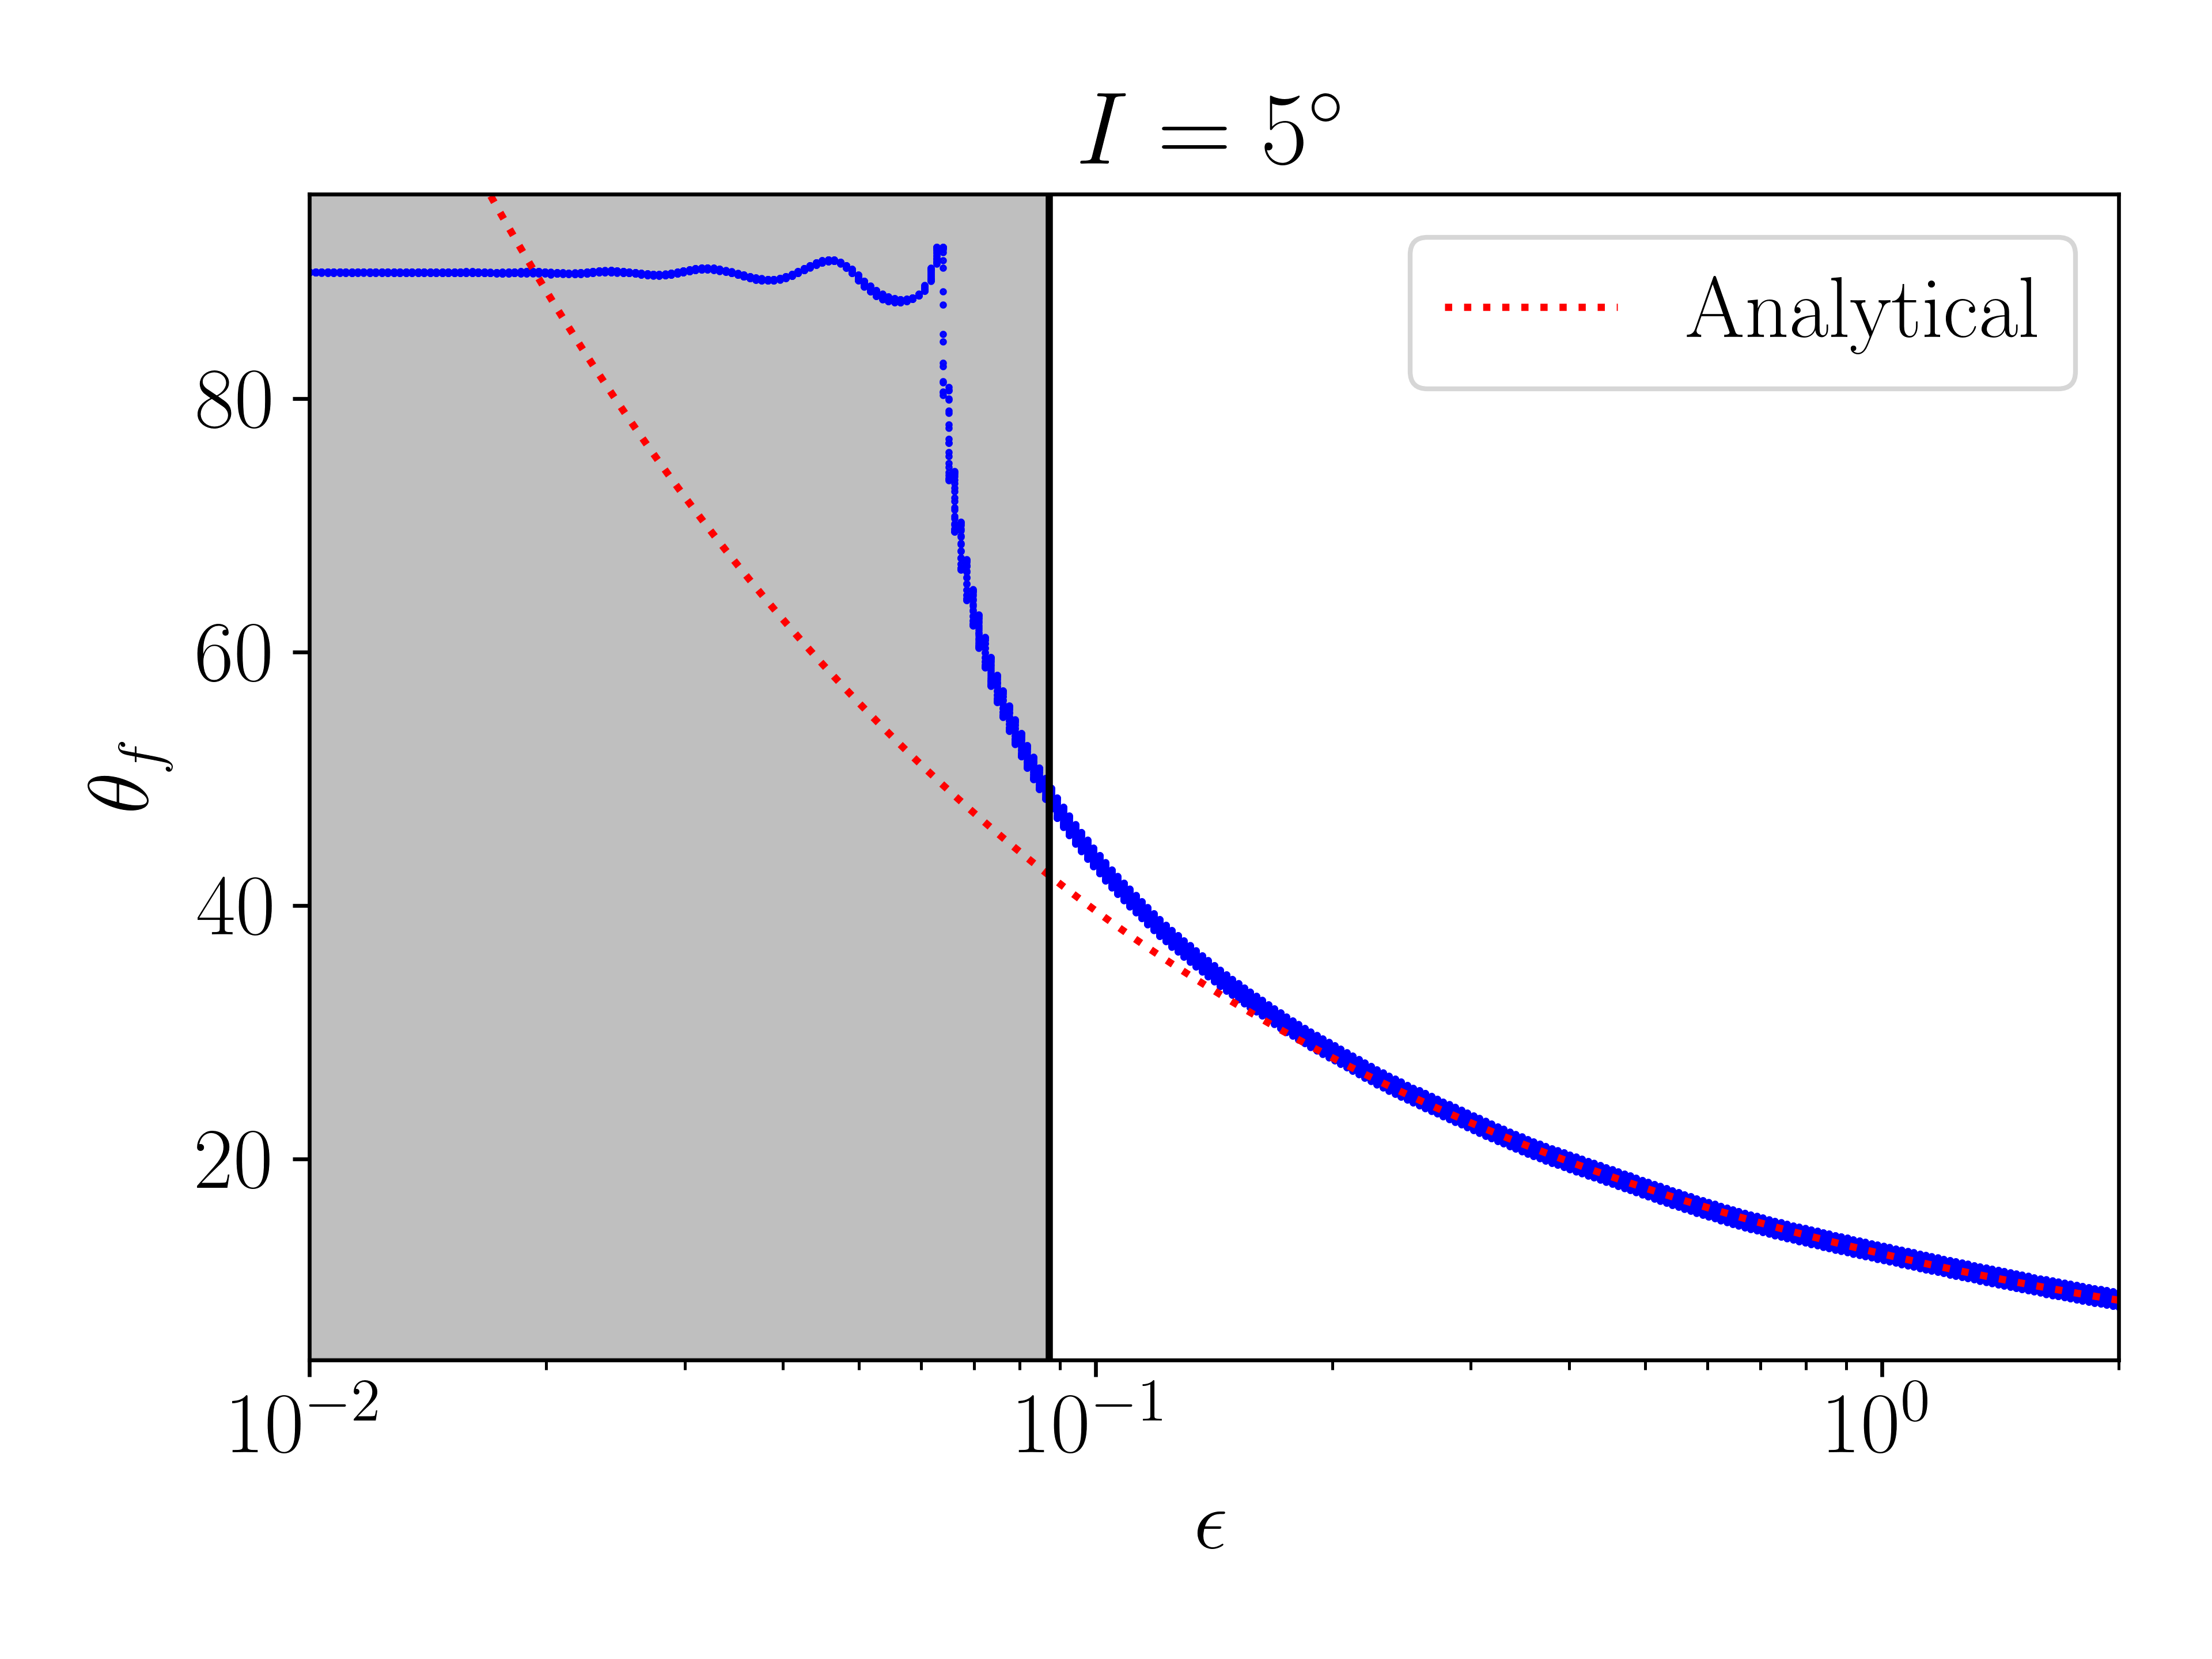
\includegraphics[width=\textwidth]{2_toy2/3scan.png}
    \end{subfigure}

    \begin{subfigure}{0.45\textwidth}
        \centering
        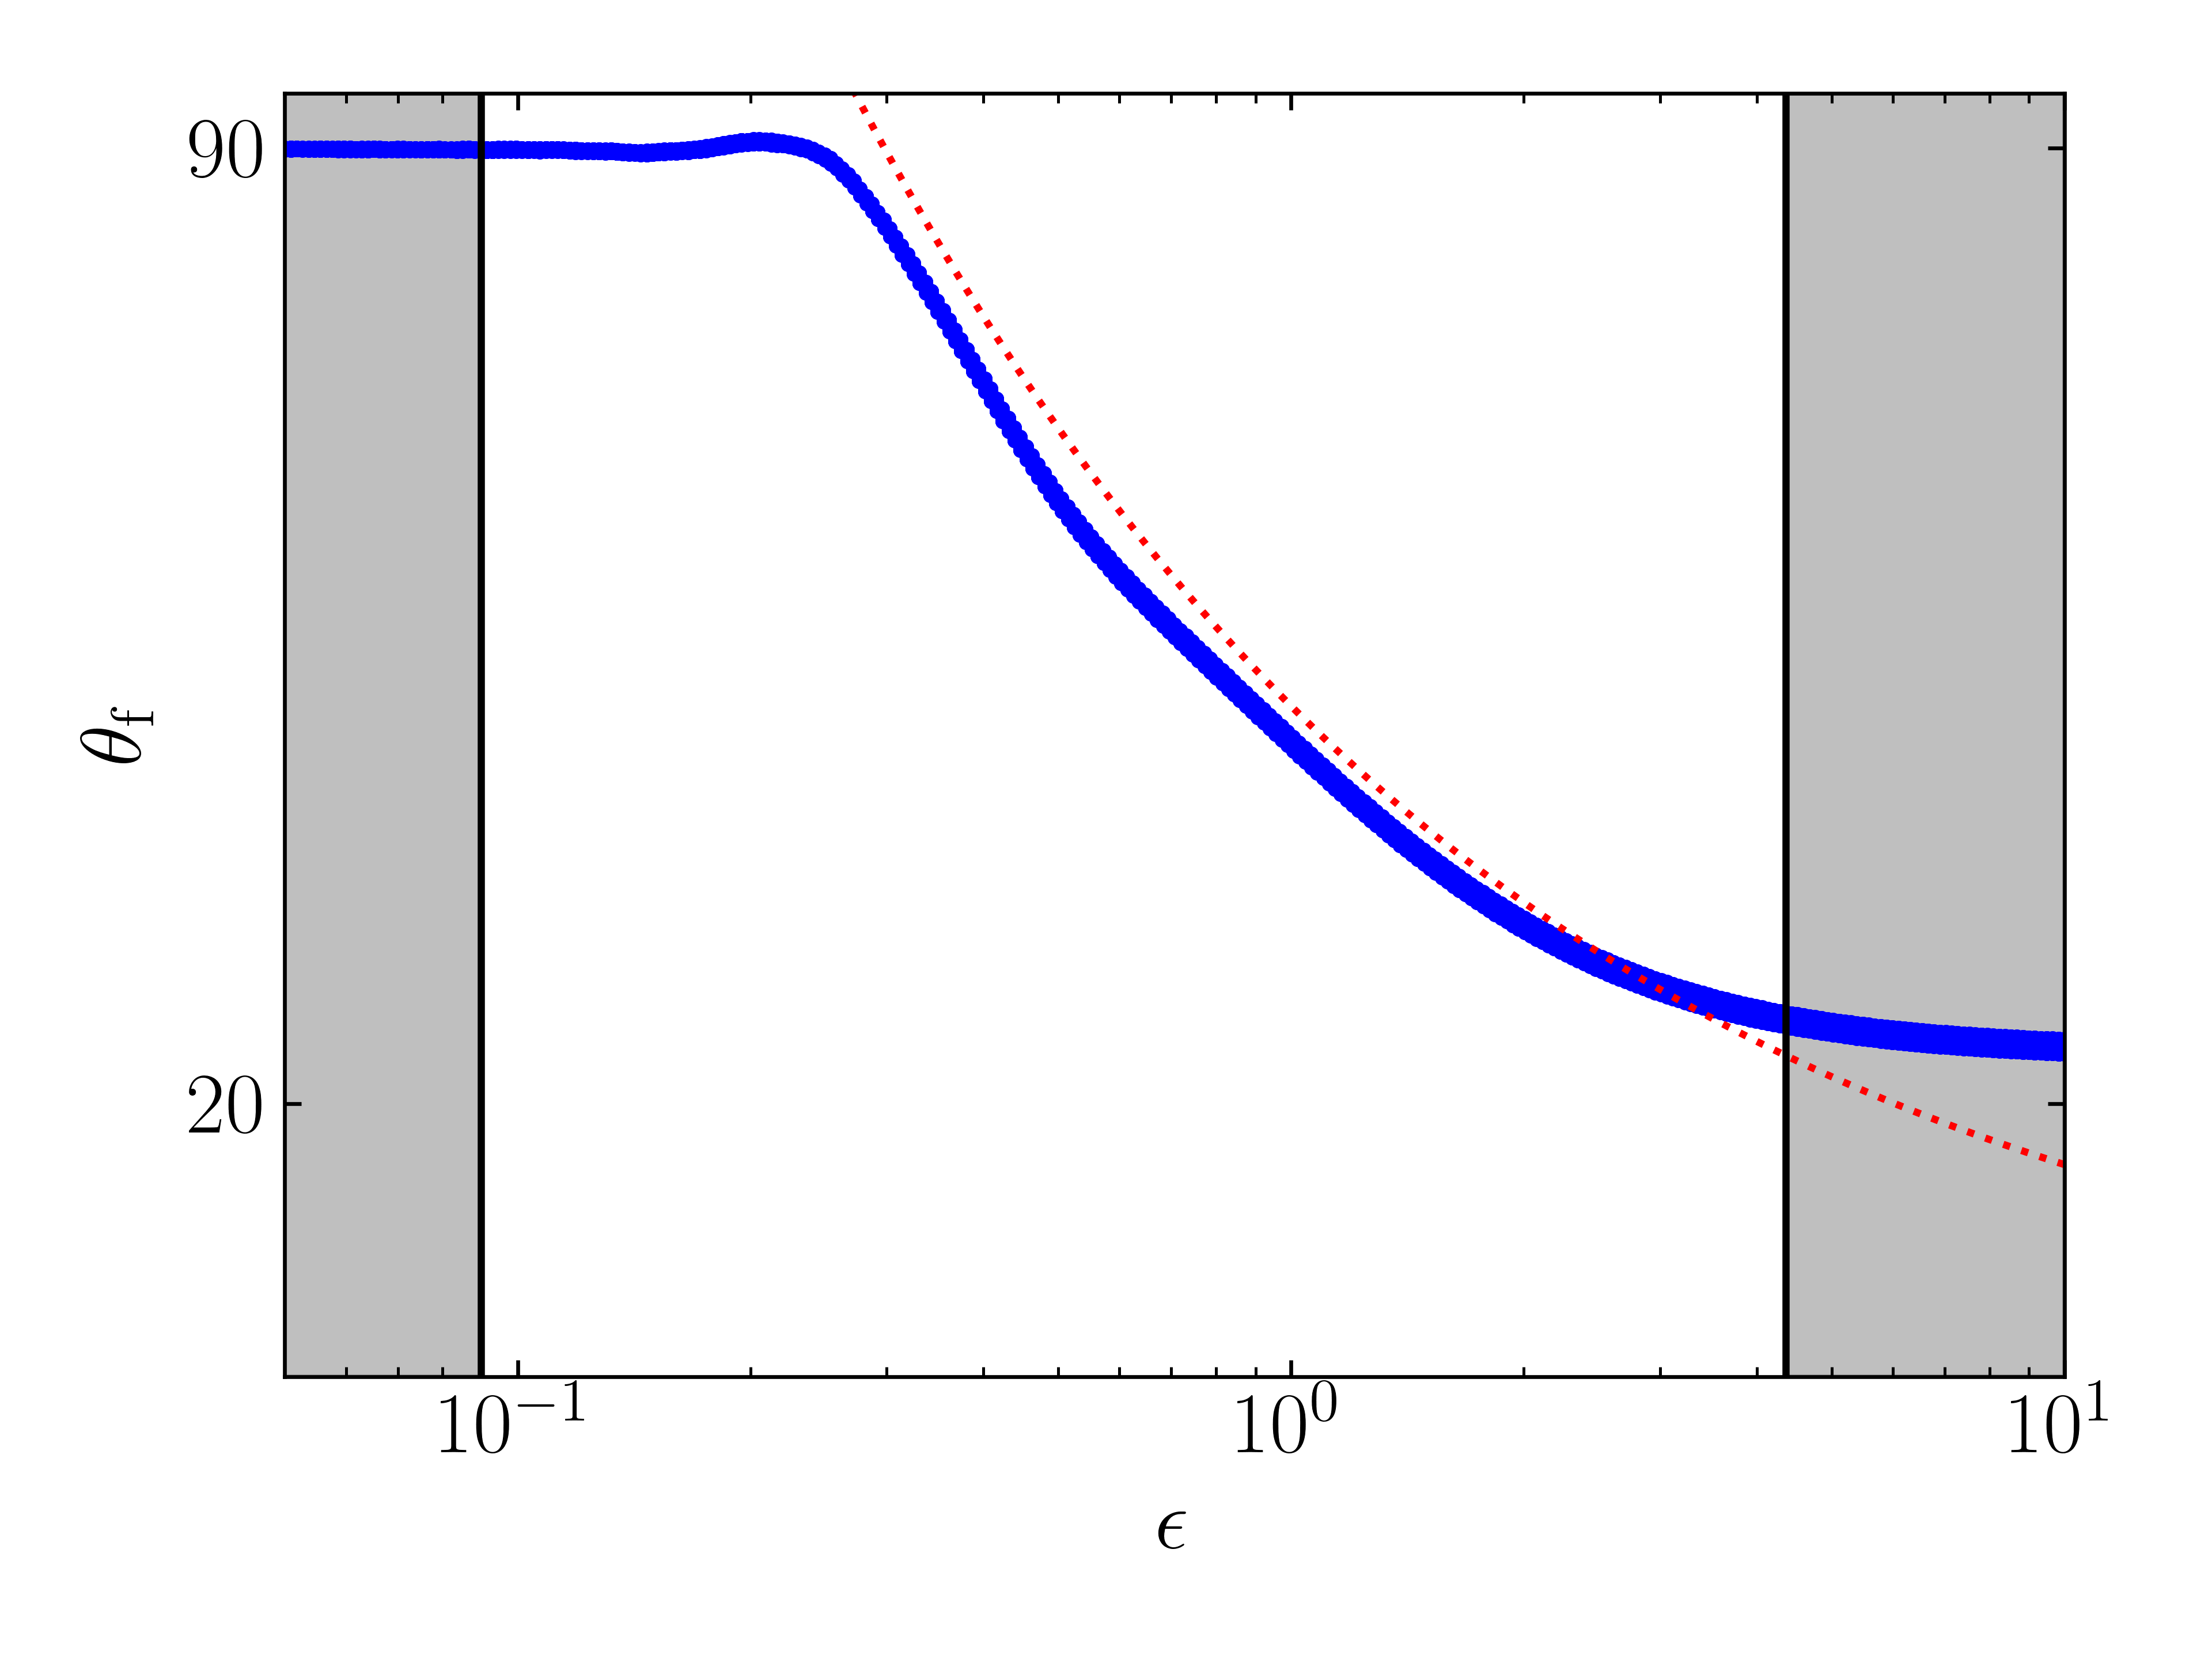
\includegraphics[width=\textwidth]{2_toy2/3scan_20.png}
    \end{subfigure}
    \caption{$I = 5^\circ, 20^\circ$ distributions vs data. Red lines are the
    result of Dong's calculation, blue are with my
    improvements.}\label{fig:nonad_scan}
\end{figure}

\subsection{Extending Dong's result}

Perhaps the easiest correction to make is, instead of assuming $s_z = 1$, to
hold it constant at $s_z \approx \cos I$, which just changes the inhomogeneous
term in \autoref{eq:nonad_ode} to $\p{-i\eta \sin I \cos I}$; this is a very
small change since $\cos I \approx 1$ for nearly all physical parameter space,
but does improve the fit slightly.

One other observation is that the LHS of \autoref{eq:nonad_int} should really be
$\abs{S\p{t}e^{i\Phi(t)} - S\p{-\infty}e^{i\Phi(-\infty)}}$, but we don't
really know $e^{i\Phi}$ since it oscillates so quickly. Thus, only when $S\p{t}
\gg S\p{-\infty}$ or $\theta_{sl, f} \gg I$ is the LHS easily evaluated. But at
the very least we can claim that $\theta_{sl, f} = \max\p{\abs{S}, I}$, so
that at very small $\abs{S}$ we just use $I$ the approximate location of CS2.
This seems to be in pretty good agreement if we look at
\lstinline{2_toy2/3Iscan} plots.

Somewhat surprisingly, using a proper $\theta_{sl, f} = \arccos 1 - S^2$
actually hurts the fit; this would manifest in the larger $\theta_{sl, f}$
regime, so it appears increasing adiabiticity dominates this correction.

The other correction to consider is how the nonadiabatic assumption breaks down.
In the stationary phase integral, we assumed that the phase could be integrated
as an imaginary Gaussian.

\textbf{Take 1 (fail):} This is only true if the in the
vicinity of the minimum, $\Phi(t)$ is approximately symmetric. The ``vicinity''
here is defined as where $\Phi(t) \lesssim \Phi_{\min} + 2\pi$, since that is
where the phase begins to oscillate quickly again. To simplify, we can write
$\eta = e^{-\epsilon t}/\cos I$, then we can integrate analytically:
\begin{equation}
    \Phi(t) = t + \frac{e^{-\epsilon t}}{\epsilon}
        \approx \frac{1}{\epsilon} + t - te^{-\epsilon t} + \mathcal{O}(t^2).
\end{equation}
can be written down analytically, we can examine how symmetric $\Phi$ is about
its minimum. It turns out though that $\Phi$ is actually \emph{more} symmetric
for smaller $\epsilon$, so stationary phase should work \emph{better}. Hm.
Similar arguments can be constructed for $\Phi$ being symmetric about $\pm
\sigma \sim 1/\sqrt{\epsilon}$, or for the variation of $\eta$ across $t \in \pm
1/\sqrt{\epsilon}$, but they all seem to favor smaller $\epsilon$ being more
accurate.

\textbf{Millholland Non-Adiabiticity:} The criterion for adiabiticity presented
in Millholland \& Batygin \emph{Primordial Obliquities} is (their Equation 15)
\begin{equation}
    \dot{\alpha} - \dot{g} \lesssim \alpha g \sin \theta \sin I.
\end{equation}
Noting $\dot{\eta} = \p{\frac{\dot{g}}{g} - \frac{\dot{\alpha}}{\alpha}}\eta$,
where $\eta = \frac{g\cos I}{\alpha}$ ($g, \alpha$ follow their definitions),
and that at crossing they define $g \approx \alpha$, then
\begin{align*}
    \frac{\dot{\alpha}}{\alpha} - \frac{\dot{g}}{g}
        &\lesssim g\sin\theta\sin I,\\
    -\s{\frac{\dot{\alpha}}{\alpha} - \frac{\dot{g}}{g}}\cos I = \dot{\eta}
        = -\epsilon \alpha \eta &\gtrsim -g\sin\theta\sin I\cos I,\\
    \epsilon &\lesssim \frac{\sin \theta \sin I \cos I}{\eta}
        \approx \sin\theta \sin I.
\end{align*}
This is overplotted in the vertical blue line in \autoref{fig:nonad_scan}.

\section{Misc}

\subsection{Another Set of Canonical Coordinates}

Consider canonical coordinates $x = 2\sin \frac{\theta}{2}\cos \phi, y = 2\sin
\frac{\theta}{2}\sin \phi$ (these can be verified to be canonical by evaluating
PB $\z{y, x}_{\cos \theta, \phi} = 1$), then the Hamiltonian can be written
\begin{align}
    H &= -\frac{1}{2}\cos^2\theta
        + \eta \p{\cos \theta \cos I - \sin I \sin \theta \cos \phi}
        ,\nonumber\\
        &= -\frac{1}{2}\p{1 - 2\sin^2\frac{\theta}{2}}^2
            + \eta\p{\p{1 - 2\sin^2\frac{\theta}{2}}\cos I
            - 2 \sin \frac{\theta}{2}\cos \phi \cos \frac{\theta}{2}\sin I}
            ,\nonumber\\
        &= -\frac{1}{2}\p{1 - \frac{x^2 + y^2}{2}}^2
            + \eta\p{\p{1 - \frac{x^2 + y^2}{2}}\cos I
                - \sin I x\sqrt{1 - \frac{x^2 + y^2}{4}}}.
\end{align}
This is in agreement w/ Millholland \& Batygin 2019's Eq.~26. These have EOM
\begin{align*}
    \dot{y} = -\pd{H}{x} &=
        -x\p{1 - \frac{x^2 + y^2}{2}} - \eta\p{
            -x \cos I + \frac{x^2\sin I}{4}\p{1 - \frac{x^2 + y^2}{4}}^{-1/2}
            - \sin I \sqrt{1 - \frac{x^2 + y^2}{4}}},\\
    \dot{x} = \pd{H}{y} &=
        y\p{1 - \frac{x^2 + y^2}{2}} + \eta\p{
            -y \cos I + \frac{xy\sin I}{4}\p{1 - \frac{x^2 + y^2}{4}}^{-1/2}
            },\\
\end{align*}
The signs can be confirmed by considering that $\theta, x, y \approx 0$ in the
$\eta \to 0$ limit results in $\dot{\phi} < 0$, or at $\phi \approx 0, y \propto
\sin \phi \propto \phi$ and $\dot{y} < 0$. It bears noting that $x^2 + y^2 \in
[0, 4]$, so the EOM diverge as $\theta \to \pi$. This is one fewer singularity
than the naive $\p{\cos\theta, \phi}$ covering, but full cartesian $\hat{s} =
\p{s_x, s_y, s_z}$ still has no singularities.

\subsection{Destruction of CS via Tides}

Let's return to the simple EOM considered in the constant $\eta$ tides case,
where
\begin{align}
    \pd{\phi}{t} &= -\mu + \eta\p{\cos I + \sin I \frac{\mu}{\sqrt{1 - \mu^2}}
        \cos \phi} ,\\
    \pd{\mu}{t} &= -\eta \sin I \sin \phi + \s{\epsilon \p{1 - \mu^2}},
\end{align}
We want to determine where tides destroys CS2. We saw before that tides tends to
shift CS2/CS4 towards each other. In fact, we can immediately see where they
will collide: in the $\dot{\mu}$ equation, no $\phi$ is stationary if
\begin{equation}
    \epsilon > \frac{\eta \sin I}{1 - \mu^2}.
\end{equation}
Note that we can invert this to find, for a given $\epsilon$, the smallest value
of $\eta$ for which CS2 is still stable, which must satisfy $\eta \sin I =
\epsilon\p{1 - \eta^2\cos^2 I}$, or
\begin{equation}
    \eta_{\min} \equiv \frac{-\sin I + \sqrt{\sin^2I
            + 4\epsilon^2 \cos^2 I}}{2\epsilon \cos^2 I}
        \approx \frac{2\epsilon^2 \cos^2 I / \sin^2 I}{
            2\epsilon \cos^2 I}
        = \frac{\epsilon}{\sin^2 I}.
\end{equation}

We can substitute in $\mu_2, \mu_4 \sim \eta \cos I$ to obtain
\begin{equation}
    \epsilon_{c} \approx \frac{\eta \sin I}{1 - \eta^2\cos^2 I}.
\end{equation}

Of course, we can also solve perturbatively to higher order for the corrections
to CS2/CS4 about their $\epsilon = 0$ values; we have already found before the
first order correction to $\phi$
\begin{equation}
    \phi_{4, 2} = \z{0, \pi} \pm \frac{\epsilon\p{1 - \mu^2}}{\eta \sin I}
        \approx \z{0, \pi} \pm \frac{\epsilon}{\eta \sin I} +
        \mathcal{O}\p{\epsilon^2}.
\end{equation}
This can then be substituted back in to find the correction to $\mu_{4, 2}$
\begin{equation}
    \mu_{4, 2} \approx \frac{\eta \cos I}{1 \mp \eta \sin I}
        \mp \frac{1}{2}\frac{\eta^2 \sin I \cos I}{1 \mp \eta \sin I}
            \p{\frac{\epsilon}{\eta \sin I}}^2 + \mathcal{O}\p{\epsilon^3}.
\end{equation}
These corrections and $\epsilon_c$ can be found in good agreement w/ numerics in
\lstinline{99_misc/0_stab.png}.

In fact, we can really do better: just let $\sin \phi = \frac{\epsilon\p{1 -
z_0^2}}{\eta \sin I}$, then $\mu = \frac{\eta \cos I}{1 - \eta \sin I \cos \phi
\frac{1}{\sqrt{1 - z_0}}}$ where $z_0 = \eta \cos I$ is the zeroth order
estimate. This is what is plotted in the aforementioned plot.

Now, a slightly more subtle question: is it possible for CS2 to still exist but
lose stability? Consider that for some $\epsilon\lesssim \epsilon_c$, the
equilibria lie at $\phi_{2, 4} = \pi/2 \pm \Delta \phi$, where $\epsilon_c -
\epsilon = \eta \sin I \frac{\Delta \phi^2}{2}$, then we consider perturbation
about these equilibria $\phi_{2, 4} = \pi/2 \pm \Delta \phi + \delta \phi$. The
linearized equations then read
\begin{subequations}
    \begin{align}
        \dot{\phi} &\approx -\delta \mu \mp \eta^2 \sin I \cos I \delta \phi,\\
        \dot{\mu} &\approx \pm\eta \sin I \Delta \phi \delta \phi.
    \end{align}
\end{subequations}
The eigenvalue equation for this first-order system reads
\begin{equation}
    \lambda^2 \pm \eta^2 \sin I \cos I \pm \eta \sin I \Delta \phi = 0.
\end{equation}
This has real solutions if
\begin{equation}
    \p{\eta^2 \sin I \cos I}^2 \mp \eta \sin I \Delta \phi > 0.
\end{equation}
If $\epsilon \sim \epsilon_c / 2$, i.e.\ not too close to critical, then
$\Delta \phi^2 \sim 1$, so except for $\epsilon_c - \epsilon \ll \epsilon_c$,
the second term dominates the first and we have one real and one imaginary root,
corresponding to the two CSs. Otherwise, we can identify that for
\begin{align*}
    \Delta \phi &\leq \eta^3 \sin I \cos^2 I,\\
    \epsilon_c - \epsilon &\leq \frac{\eta^7 \sin^3 I \cos^4 I}{2},
\end{align*}
the eigenvalues become real. However, for CS2, since the eigenvalue equation
reads $\lambda^2 + b\lambda + c = 0$ and the eigenvalues take form $\p{-b \pm
\sqrt{b^2 - 4c}}/2$, no eigenvalue w/ positive real part ever appears, so it
remains forever stable. We can also numerically validate this via
\lstinline{99_misc/0_stab.py}.

We can illustrate the trajectories at $\phi_{2, \epsilon}$ when turning on
$\epsilon$ by examining \lstinline{99_misc/3_trajs.py}.

\subsection{Dissipating Disk: $\theta_f$ Distribution}

Consider if $\eta$ crosses $\eta_c$ with $\eta(t = 0) > \eta_c$, and there is no
dissipation, only variation of $\eta$. The area contained within the separatrix
when it first forms is given in Ward \& Hamilton Paper I\@:
\begin{equation}
    A_{crit} = 4\pi \s{1 - \p{1 + \tan^{2/3}I}^{-3/2}}.
\end{equation}
We are interested in states that start nearly aligned w/ the disk, so in Zone II
by our designation. Then, once three states appear, Zone II continues to shrink
until separatrix crossing occurs, which is at $J_i = A_2$. At the time of
separatrix crossing, the trajectory is ejected into either Zone I/III (if Zone
III is shrinking, then exclusively Zone I\@; can analytically state using
Henrard \& Murigande 1987). The possible values for the new action of the
ejected state are either $J_f = A_2 + A_3 - 2\pi$ or $J_f = A_3 - 2\pi$, when
integrating $\mu\;\mathrm{d}\phi$. From here, the states will precess uniformly
at some $\theta_f = J_f / 2\pi$.

We can investigate the values of $\theta_f$ given some initial mutual
inclination $\hat{s} \cdot \hat{l}_p \equiv \theta_{sp, i}$ ($J_i = 2\pi\p{1 -
\cos \epsilon}$ where $\epsilon$ is the initial mutual inclination). To do this,
we need to understand what the possible transitions are. When the separatrix
first appears to the final state, the transitions are $A_2 \to A_3, A_2 \to A_1,
A_3 \to A_1, A_3 \to A_2 \to A_1, A_3 \to A_3$. Let's reproduce the analytical
forms of these three areas below:
\begin{subequations}
    \begin{align*}
        z_0 &= \eta\cos I &
        \chi &= \sqrt{-\frac{\tan^3\theta_4}{\tan I} - 1},\\
        \rho &= \chi \frac{\sin^2 \theta_4\cos \theta_4}{
            \chi^2 \cos^2\theta_4 + 1} &
        T &= 2\chi \frac{\cos \theta_4}{
            \chi^2 \cos^2\theta_4 - 1},
    \end{align*}
    \begin{align}
        A_2 &= 8\rho + 4\arctan T - 8z_0 \arctan \frac{1}{\chi},\\
        A_1 &= 2\pi\p{1 - z_0} - \frac{A_2}{2},\\
        A_3 &= 2\pi\p{1 + z_0} - \frac{A_2}{2}.
    \end{align}
\end{subequations}
To determine which of the transition histories we fall under (to get an
analytical prediction for $\cos \theta_f$), we need to determine $\eta_\star$,
so we know how the enclosed $J$ by the trajectory changes due to separatrix
encounter. A guess for numerical root-finding can be put together for
trajectories that encounter from $A_2$ via (inverting the separatrix area
formula for small $\eta$)
\begin{equation*}
    \eta_\star\p{A_2} = \p{A_2/16}^2 / \sin I,
\end{equation*}
while for trajectories that encounter from $A_3$ we can solve the quadratic $A_3
= 2\pi \eta \cos I - 8\sqrt{\eta \sin I} = 4\pi - J$ and obtain
\begin{equation*}
    \sqrt{\eta_\star} = \frac{4\sqrt{\sin I} + \sqrt{16\sin I + 2\pi \cos I
        A_3}}{ 2\pi \cos I}.
\end{equation*}
This will often run over $\eta_c$, so we guess the smaller of $\eta_\star,
\eta_c$.

Finally, the $A_3 \to A_2 \to A_1$ pipeline only exists if $ \eta_{A2\max} <
\eta_\star < \eta_c$, the $\eta$ at which $A_2$ is maximized (this maximization
behavior is not captured in my linearized formulas, but can be seen in
\lstinline{99_misc/1_areas.png}). Then, two separatrix crossings occur. Thus, for
the five possible trajectories, we have the following transitions:
\begin{itemize}
    \item $A_2 \to A_3$: This transition happens with probability $\frac{-2\pi
        \eta_{\star} \cos I + 4\sqrt{\eta_{\star}\sin
        I}}{8\sqrt{\eta_{\star}\sin I}}$, so for $0 \leq \eta_{\star} \leq
        \frac{4\sin I}{\pi^2 \cos^2 I}$ this transition is permitted. The
        approximate $\mu_f$ can be estimated by conservation of adiabatic
        invariant
        \begin{align*}
            \eta_\star &\approx \p{\frac{2\pi\p{1 - \cos \theta_{sp,i}}}{
                        16}}^2 / \sin I&
                    &\approx \p{\frac{\pi \theta_{sp, i}^2}{16}}^2/\sin I,\\
            \mu_{f, 23} &\approx \eta_\star \cos I
                    - \frac{4\sqrt{\eta_\star \sin I}}{\pi} &
                &\approx\p{\frac{\pi \theta_{sp, i}^2}{16}}^2 \cot I
                    - \frac{\theta_{sp, i}^2}{4}.
        \end{align*}

    \item $A_2 \to A_1$: This transition happens with probability $\frac{-2\pi
        \eta_{\star} \cos I + 4\sqrt{\eta_{\star}\sin
        I}}{8\sqrt{\eta_{\star}\sin I}}$ and can happen so long as $\theta_{sp,
        i}$ is small enough to fit inside $A_{crit}$ when the separatrix first
        appears, i.e.\ $2\pi\p{1 - \cos \theta_{sl, i}} < A_{crit}$ (where
        $\theta_{sl, i}$ is defined in the $\eta \to \infty$ limit, and since
        there is no separatrix the enclosed area is conserved as $\eta$
        approaches $\eta_c$ from above).

        The resulting formulas for $\mu_{f, 21}$ are very similar to those above
        \begin{align*}
            \eta_\star &\approx \p{\frac{2\pi\p{1 - \cos \theta_{sp,i}}}{
                        16}}^2 / \sin I&
                    &\approx \p{\frac{\pi \theta_{sp, i}^2}{16}}^2/\sin I,\\
            \mu_{f, 21} &\approx \eta_\star \cos I
                    + \frac{4\sqrt{\eta_\star \sin I}}{\pi} &
                &\approx\p{\frac{\pi \theta_{sp, i}^2}{16}}^2 \cot I
                    + \frac{\theta_{sp, i}^2}{4}.
        \end{align*}

    \item $A_3 \to A_3$: This transition occurs if $J_i(\theta_{sl, i}) > 4\pi -
        A_{3, \min}$. This implies the circulation never undergoes a separatrix
        encounter at all, so it remains in $A_3$ forever.

    \item $A_3 \to A_1$: This transition occurs when $\theta_{sl, i}$ satisfies
        $2\pi\p{1 - \cos \theta_{sl, i}} > A_{crit}$, so the trajectory starts
        in $A_3$. It then has probability to hop to $A_1$ (TODO).

    \item $A_3 \to A_2 \to A_1$: This transition also occurs when $J_i$ is
        $> A_{crit}$, but has one further requirement, that $\eta_{\star} >
        \argmax A_2(\eta)$, such that $A_2$ is expanding during the first
        separatrix encounter. The bound on this is not exactly analytic though.
\end{itemize}

\end{document}

